\chapter{Fondements théoriques : convolution et base de Fourier}

\section{Objectif de cette section}

Cette section a pour objectif de reconstruire le raisonnement théorique proposé par 
Tsuzuku et Sato~\cite{tsuzuku2019structural}. Il s'agit de comprendre pourquoi les réseaux convolutionnels 
présentent une sensibilité particulière à certaines directions de la base de Fourier, en caractérisant mathématiquement 
ces vulnérabilités.

L'idée générale repose sur la structure mathématique des couches convolutionnelles. 
Pour l'étudier, nous nous placerons dans un cadre linéaire simplifié, en faisant fi des éléments 
classiquement introduits le long du processus de décision d'un CNN pour en briser la linéarité 
(tels que les fonctions d'activation non linéaires et le \textit{max-pooling}).

Les développements qui suivent utilisent deux rappels classiques d'algèbre linéaire :
la représentation matricielle d'une application linéaire, et le lien entre vecteurs propres,
valeurs propres et diagonalisation. Ces rappels sont donnés en annexes~\ref{app:representation-lineaire-matrice}
et~\ref{app:vecteurs-propres-diagonalisation}.

\section{Conventions de Fourier et de vectorisation}
\label{sec:conventions-fourier-vectorisation}

Avant d'étudier les convolutions, nous fixons les conventions utilisées dans tout le chapitre.

Dans la suite, toutes les fréquences et tous les indices spatiaux seront interprétés modulo $N$.

\subsection{Base de Fourier 1D et transformée discrète}

Pour un entier $N \geq 1$, on note
\[
    \mathbb{Z}_N = \{0,\dots,N-1\}
\]
l'ensemble des indices pris modulo $N$. Concrètement, cela signifie que l'indice $N$ est identifié
à l'indice $0$, l'indice $N+1$ à l'indice $1$, et ainsi de suite. Cette convention sera utilisée dans
tout le chapitre.

Pour chaque fréquence $k\in\mathbb{Z}_N$, on définit le vecteur de Fourier discret normalisé
\begin{equation}
    \phi_k[n]
    =
    \frac{1}{\sqrt{N}}
    e^{2\pi i kn/N},
    \qquad n\in\mathbb{Z}_N.
    \label{eq:def_base_fourier_1d}
\end{equation}
Le vecteur $\phi_k$ représente une onde discrète de fréquence $k$. Les petites valeurs de $k$
correspondent à des variations lentes, tandis que les fréquences plus élevées correspondent à des
oscillations plus rapides sur les $N$ points du signal. Le facteur $1/\sqrt{N}$ sert à normaliser le
vecteur, ce qui donne
\[
    \|\phi_k\|_2 = 1.
\]

On regroupe tous ces vecteurs dans une même matrice :
\begin{equation}
    F_N
    =
    \begin{pmatrix}
    | & | &        & | \\
    \phi_0 & \phi_1 & \cdots & \phi_{N-1} \\
    | & | &        & |
    \end{pmatrix}.
    \label{eq:def_matrice_fourier_1d}
\end{equation}
La matrice $F_N$ contient donc, colonne par colonne, toutes les directions de Fourier possibles
pour un signal de taille $N$. Avec la normalisation choisie, ses colonnes forment une base
orthonormée de $\mathbb{C}^N$, c'est-à-dire
\[
    F_N^H F_N = I_N,
    \qquad
    F_N^{-1}=F_N^H.
\]

La transformée de Fourier discrète consiste alors à exprimer un signal
$x\in\mathbb{C}^N$ dans cette base. Avec notre convention, les coefficients de Fourier de $x$ sont
donnés par
\begin{equation}
    \widehat{x}
    =
    F_N^H x,
\end{equation}
c'est-à-dire, composante par composante,
\begin{equation}
    \widehat{x}[k]
    =
    \frac{1}{\sqrt{N}}
    \sum_{n=0}^{N-1}
    x[n]e^{-2\pi i kn/N}.
    \label{eq:def_dft_1d}
\end{equation}
Le coefficient $\widehat{x}[k]$ mesure la contribution de la fréquence $k$ dans le signal.

Comme $F_N$ est unitaire, on peut reconstruire le signal à partir de ses coefficients de Fourier par
\begin{equation}
    x
    =
    F_N\widehat{x},
\end{equation}
ou encore, composante par composante,
\begin{equation}
    x[n]
    =
    \frac{1}{\sqrt{N}}
    \sum_{k=0}^{N-1}
    \widehat{x}[k]e^{2\pi i kn/N}.
    \label{eq:def_idft_1d}
\end{equation}

\subsection{Base de Fourier 2D}

On passe maintenant des signaux 1D aux images 2D. Pour une image
$X\in\mathbb{C}^{N\times N}$, on utilise les indices spatiaux
\[
    (m,n)\in\mathbb{Z}_N^2.
\]
L'indice $m$ désigne la position verticale, et l'indice $n$ la position horizontale.

De la même manière, une fréquence 2D est décrite par un couple
\[
    (u,v)\in\mathbb{Z}_N^2.
\]
L'indice $u$ correspond à la fréquence verticale, tandis que l'indice $v$ correspond à la fréquence
horizontale.

Pour chaque couple de fréquences $(u,v)$, on définit l'image de Fourier 2D
\begin{equation}
    \Phi_{u,v}[m,n]
    =
    \phi_u[m]\phi_v[n]
    =
    \frac{1}{N}
    e^{2\pi i(um+vn)/N}.
    \label{eq:def_base_fourier_2d}
\end{equation}
Cette formule signifie qu'une onde de Fourier 2D est obtenue comme le produit d'une onde verticale
et d'une onde horizontale sous forme matricielle : $\Phi_{u,v} = \phi_u \phi_v^T$.

En faisant varier les fréquences $u$ et $v$, on obtient différents motifs périodiques dans l'espace
des images. Visuellement, ces motifs peuvent prendre la forme de bandes, de grilles ou d'oscillations
orientées, dont la densité dépend directement du couple $(u,v)$. Ainsi, ajouter une direction de
Fourier à une image revient à lui superposer un motif géométrique périodique.

\begin{figure}[H]
    \centering
    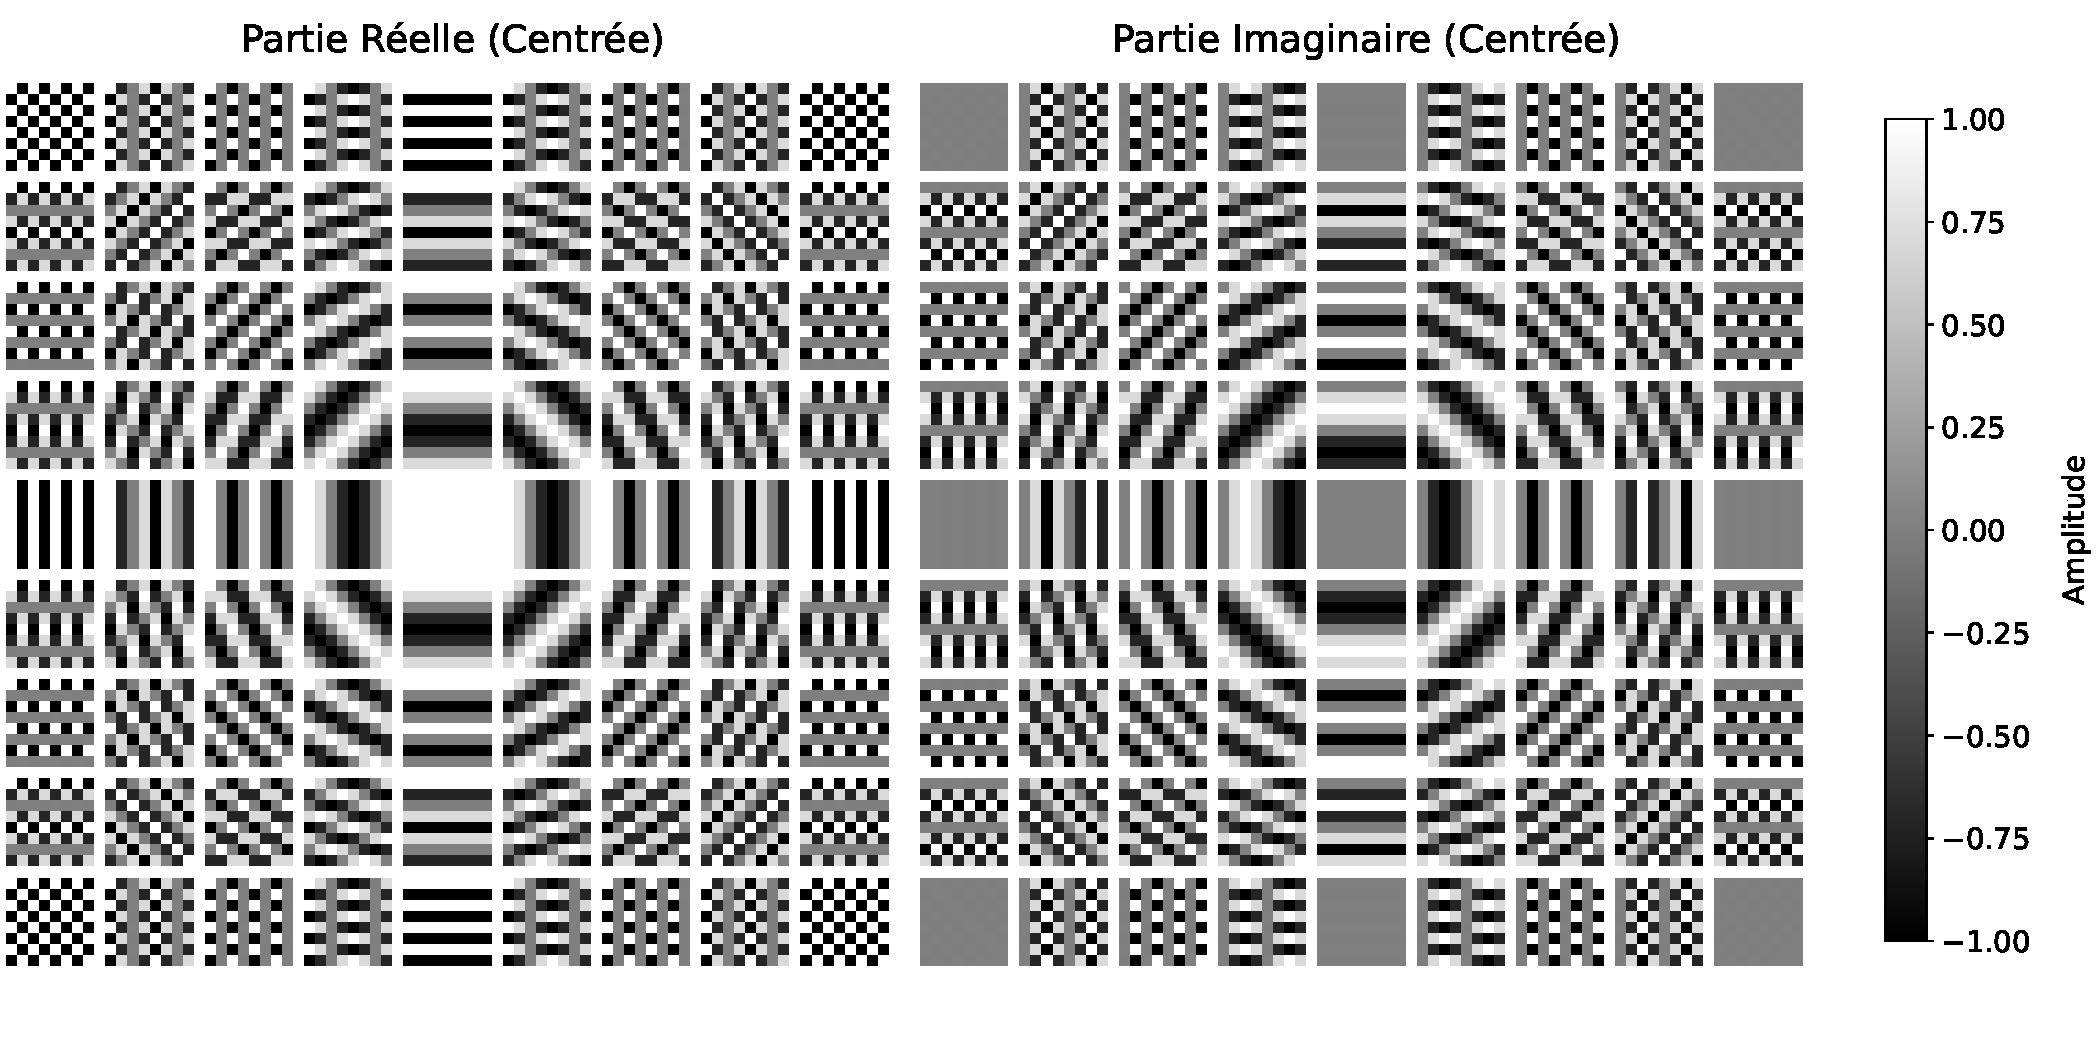
\includegraphics[width=0.95\textwidth]{figures/theory/fourier_basis_2d.pdf}
    \caption{Visualisation des bases de Fourier 2D pour tous les couples de fréquences $(u,v)$ d'une image de taille $9 \times 9$. La partie réelle et la partie imaginaire sont affichées séparément. Les basses fréquences sont situées au centre des grilles, tandis que les hautes fréquences se trouvent en périphérie.}
    \label{fig:fourier_basis_2d}
\end{figure}

Dans les figures, on représentera parfois les fréquences de manière centrée, avec les basses fréquences
au centre de l'image. Cette convention est pratique pour la visualisation. En revanche, dans les formules,
les indices restent toujours dans $\{0,\dots,N-1\}$ et sont interprétés modulo $N$.

\subsection{Vectorisation et produit de Kronecker}

Dans tout le chapitre, nous vectorisons les images en empilant les colonnes. Pour
$X\in\mathbb{C}^{N\times N}$, on pose donc
\begin{equation}
\operatorname{vec}(X)
=
\begin{pmatrix}
X[0,0] \\
X[1,0] \\
\vdots \\
X[N-1,0] \\
X[0,1] \\
\vdots \\
X[N-1,N-1]
\end{pmatrix}.
\label{eq:def_vectorisation_colonnes}
\end{equation}
On lit d'abord la première colonne, puis la deuxième, et ainsi de suite. Avec cette convention,
l'entrée $X[m,n]$ correspond à l'indice vectorisé
\[
    m+Nn.
\]

Nous utiliserons aussi le produit de Kronecker, noté $\otimes$. Défini comme suit, soient
$A \in \mathbb{C}^{m \times n}$ et $B \in \mathbb{C}^{p \times q}$, alors la matrice par blocs de taille
$mp \times nq$ est définie par

$$
A \otimes B =
\begin{pmatrix}
a_{11}B & a_{12}B & \cdots & a_{1n}B \\
a_{21}B & a_{22}B & \cdots & a_{2n}B \\
\vdots  & \vdots  & \ddots & \vdots  \\
a_{m1}B & a_{m2}B & \cdots & a_{mn}B
\end{pmatrix}.
$$

Il permet notamment de construire
une base de Fourier 2D à partir de deux bases de Fourier 1D. Les propriétés algébriques de la
vectorisation et du produit de Kronecker sont déjà connues en analyse matricielle~\cite{horn2013matrix}.

Avec notre convention de vectorisation par colonnes, on a en particulier
\begin{equation}
    \operatorname{vec}(ab^T)
    =
    b\otimes a.
    \label{eq:vec_produit_exterieur}
\end{equation}

En appliquant cette identité à l'image de Fourier
\[
    \Phi_{u,v}=\phi_u\phi_v^T,
\]
on obtient
\begin{equation}
    \operatorname{vec}(\Phi_{u,v})
    =
    \phi_v\otimes\phi_u.
    \label{eq:vec_fourier_2d}
\end{equation}
Ainsi, dans toute la suite du chapitre, la colonne de $Q_N$ associée à la fréquence 2D $(u,v)$ sera notée
\[
    q_{u,v}
    =
    \phi_v\otimes\phi_u.
\]

On note alors
\begin{equation}
    Q_N = F_N \otimes F_N
    \label{eq:def_base_fourier_2d_vectorisee}
\end{equation}
la base de Fourier 2D vectorisée. Par unitarité de $F_N$ :
\[
    Q_N^H Q_N = I_{N^2}.
\]
Les colonnes de $Q_N$ forment donc une base orthonormée de $\mathbb{C}^{N^2}$.

Avec la notation précédente, la colonne associée à la fréquence $(u,v)$ est
\[
    (Q_N)_{w(u,v)}
    =
    q_{u,v}
    =
    \phi_v\otimes\phi_u.
\]
L'indice $w(u,v)$ est simplement l'indice aplati qui permet de passer du couple de fréquences
$(u,v)$ à un seul indice de colonne dans $Q_N$. Il est défini par
\begin{equation}
    w(u,v)=u+Nv.
    \label{eq:indice_frequence_aplati}
\end{equation}\

Réciproquement, si l'on connaît un indice aplati $w\in\{0,\dots,N^2-1\}$, on retrouve le couple
de fréquences correspondant par
\[
    u = w \bmod N,
    \qquad
    v = \left\lfloor \frac{w}{N} \right\rfloor.
\]

\section{Convolution discrète en dimension 1}

Avant d'étudier les images, nous commençons par le cas plus simple d'un signal discret périodique représenté 
par sa période $x = (x[0], x[1], \ldots, x[N-1])$ avec $x[i] \in \mathbb{R}$.
Soit $x \in \mathbb{R}^N$ notre signal et $h = (h[0], h[1], \ldots, h[N-1]) \in \mathbb{R}^N$ notre filtre (qui sera 
supposé de même taille que le signal, quitte à être complété par des zéros). 
La convolution circulaire entre $h$ et $x$ est définie par :

\[
y[n] = (h * x)[n] = \sum_{k=0}^{N-1} h[k]\,x[(n-k) \bmod N] \text{~\cite{ImagerieNumeriqueTheme7Block2}}
\]

L'opération modulo signifie que les indices du signal sont pris dans 
\(\mathbb{Z}_N\). 
Ainsi, lorsqu'un indice sort de l'intervalle \(\{0,\ldots,N-1\}\), 
il est ramené à sa classe correspondante dans \(\mathbb{Z}_N\).
Le signal est donc interprété comme périodique, comme l'illustre la 
figure~\ref{fig:padding_circulaire}. 

\begin{figure}[H]
    \centering
    \begin{tikzpicture}[
        node distance=0cm,
        cell/.style={rectangle, draw=black, thick, minimum width=1.2cm, minimum height=1.2cm, text centered, font=\large},
        pad/.style={rectangle, draw=gray, dashed, fill=gray!10, minimum width=1.2cm, minimum height=1.2cm, text centered, font=\large, text=gray}
    ]
    
    \node[cell] (x0) {$x_0$};
    \node[cell, right=of x0] (x1) {$x_1$};
    \node[cell, right=of x1] (x2) {$x_2$};
    \node[cell, right=of x2] (x3) {$x_3$};
    
    \node[pad, left=of x0] (pL1) {$x_3$};
    \node[pad, left=of pL1] (pL2) {$x_2$};
    
    \node[pad, right=of x3] (pR1) {$x_0$};
    \node[pad, right=of pR1] (pR2) {$x_1$};
    
    \draw [decorate,decoration={brace,amplitude=5pt,mirror}]
        (x0.south west) -- (x3.south east) node[midway,below=10pt] {Signal original $x$};
    
    \draw [decorate,decoration={brace,amplitude=5pt}, gray]
        (pL2.north west) -- (pL1.north east) node[midway,above=10pt] {\textit{Padding}};
        
    \draw [decorate,decoration={brace,amplitude=5pt}, gray]
        (pR1.north west) -- (pR2.north east) node[midway,above=10pt] {\textit{Padding}};

    \draw[->, thick, gray, dashed, bend left=45] (x3.north) to node[above] {} (pL1.north);
    \draw[->, thick, gray, dashed, bend right=45] (x0.south) to node[below] {} (pR1.south);

    \end{tikzpicture}
    \caption{Représentation du \textit{padding} circulaire pour un signal 1D. Les bords du signal se répètent de manière périodique.}
    \label{fig:padding_circulaire}
\end{figure}

\paragraph{Remarque sur l'hypothèse de périodicité.}

Dans cette section, nous travaillons avec des convolutions circulaires. Cela revient à considérer les
signaux comme périodiquement prolongés : lorsque l'on dépasse une extrémité du signal, on revient
de l'autre côté. Cette hypothèse est très utile mathématiquement, car elle permet de diagonaliser les
convolutions par la base de Fourier discrète.

Elle ne correspond cependant pas toujours au comportement exact des images réelles aux bords :
si les extrémités ne se raccordent pas naturellement, la périodisation peut créer une discontinuité
artificielle. Ce point est discuté plus en détail en annexe~\ref{app:periodicite-bords-gibbs}.

\section{Les fonctions de Fourier comme fonctions propres de la convolution circulaire}
\label{sec:fourier-vecteurs-propres}

\paragraph{Cas unidimensionnel}

On se place dans l'espace des signaux discrets périodiques de période $N$ :
\[
V_N = \{x : \mathbb{Z}_N \rightarrow \mathbb{C}\}.
\]
Un élément de $V_N$ peut être vu soit comme une fonction discrète périodique, soit comme un vecteur de $\mathbb{C}^N$.

Pour un filtre $h \in \mathbb{C}^N$ fixé, la convolution circulaire définit un opérateur linéaire
\[
\mathcal{C}_h : V_N \rightarrow V_N,
\qquad
\mathcal{C}_h(x) = h * x.
\]

Pour chaque fréquence $f \in \{0,\dots,N-1\}$, on utilise le vecteur de Fourier normalisé
$\phi_f$ défini en \eqref{eq:def_base_fourier_1d}.

Le résultat fondamental liant la convolution circulaire et la base de Fourier s'écrit alors :

\begin{equation}
\mathcal{C}_h(\phi_f) = \lambda_f \phi_f,
\label{eq:fourier_fonction_propre_conv_1d}
\end{equation}

c'est-à-dire, composante par composante :
\[
(h * \phi_f)[n] = \lambda_f \phi_f[n],
\]
où
\[
\lambda_f =
\sum_{k=0}^{N-1} h[k] e^{-2\mathrm{i}\pi f k/N}.
\]

Il est important de remarquer que $\lambda_f$ dépend du filtre $h$ et de la fréquence $f$,
mais pas de la position $n$. Ainsi, lorsque l'entrée de l'opérateur de convolution circulaire
est une onde de Fourier, la convolution ne modifie pas sa forme spatiale : elle se contente
de la multiplier par un scalaire complexe. Autrement dit, $\lambda_f$ est une valeur propre et
$\phi_f$ une fonction propre de l'opérateur de convolution circulaire
$\mathcal{C}_h$.

\begin{proof}
\begin{alignat*}{2}
    (\mathcal{C}_h(\phi_f))[n] &= (h * \phi_f)[n] \\
    &= \sum_{k=0}^{N-1} h[k]\,\phi_f[(n-k) \bmod N] \\
    \text{\small (périodicité de $\phi_f$)} \quad &= \sum_{k=0}^{N-1} h[k]\,\phi_f[n-k] \\
    \text{\small (propriété de l'exponentielle)} \quad &= \sum_{k=0}^{N-1} h[k] e^{-2\mathrm{i}\pi f k/N}\phi_f[n] \\
    &= \left(\sum_{k=0}^{N-1} h[k] e^{-2\mathrm{i}\pi f k/N}\right)\phi_f[n] \\
    &= \lambda_f \phi_f[n].
\end{alignat*}

\end{proof}

Ce résultat correspond au théorème de convolution discret : dans le domaine de Fourier,
une convolution circulaire devient une multiplication fréquence par fréquence. Ainsi,
lorsque l'entrée est une onde de Fourier pure \(\phi_f\), la convolution ne change pas
sa fréquence ; elle la multiplie seulement par un scalaire. On obtient donc \ref{eq:fourier_fonction_propre_conv_1d}

\subsection{Conséquence matricielle : diagonalisation des matrices circulantes}

Pour un filtre $h$ fixe, la convolution circulaire 1D définit une application linéaire de $\mathbb{C}^N \rightarrow \mathbb{C}^N$
car pour tous $x, y \in \mathbb{C}^N$ et tous $\alpha, \beta \in \mathbb{C}$ nous avons que
\begin{align*}
h * (\alpha x + \beta y) &= \alpha (h * x) + \beta (h * y)
\end{align*}

\begin{proof}
\begin{alignat*}{2}
    (h * (\alpha x + \beta y))[n] &= \sum_{k=0}^{N-1} h[k]\,(\alpha x + \beta y)[(n-k) \bmod N]  \\
    &= \sum_{k=0}^{N-1} h[k]\,(\alpha x[(n-k) \bmod N] + \beta y[(n-k) \bmod N])  \\
    &= \alpha \sum_{k=0}^{N-1} h[k]\,x[(n-k) \bmod N] + \beta \sum_{k=0}^{N-1} h[k]\,y[(n-k) \bmod N]  \\
    &= \alpha (h * x)[n] + \beta (h * y)[n].
\end{alignat*}

\end{proof}

Comme cette opération est linéaire, le rappel de l'annexe~\ref{app:representation-lineaire-matrice}
garantit qu'elle peut être représentée, une fois une base choisie, par une matrice
$C_h \in \mathbb{C}^{N \times N}$ telle que pour tout signal d'entrée $x \in \mathbb{C}^N$ :

$$
y = C_h x.
$$

où $C_h$ est une matrice circulante construite à partir du filtre $h$ telle que la première ligne est organisée de manière à reproduire $y[0]$,
puis chaque ligne suivante est obtenue par décalage circulaire :

$$
C_h =
\begin{pmatrix}
h[0] & h[N-1] & h[N-2] & \cdots & h[1] \\
h[1] & h[0] & h[N-1] & \cdots & h[2] \\
h[2] & h[1] & h[0] & \cdots & h[3] \\
\vdots & \vdots & \vdots & \ddots & \vdots \\
h[N-1] & h[N-2] & h[N-3] & \cdots & h[0]
\end{pmatrix}.
$$

En effet, $y[0] = h[0]x[0] + h[1]x[N-1] + \cdots + h[N-1]x[1]$ correspond à la première ligne de $C_h$ 
multipliée par le vecteur $x$, en appliquant itérativement la même logique on obtient les autres éléments de $y$.

\vspace{0.5cm}

En choisissant la base canonique de $\mathbb{C}^N$, l'opérateur linéaire $\mathcal{C}_h$
est représenté par la matrice circulante $C_h$. La relation
$\mathcal{C}_h(\phi_f) = \lambda_f \phi_f$ peut alors être réécrite sous forme matricielle :

\begin{equation}
    C_h \phi_f = \lambda_f \phi_f
    \label{eq:fourier_eigen_matrice}
\end{equation}

Ainsi, chaque fonction de Fourier $\phi_f$ est un vecteur propre de la matrice circulante $C_h$,
avec valeur propre associée $\lambda_f$. Ce qui signifie que dans le cadre 
circulaire, la convolution agit diagonalement dans la base de Fourier.

En utilisant la matrice de Fourier $F_N$ définie en \eqref{eq:def_matrice_fourier_1d},
on regroupe les valeurs propres dans la matrice diagonale :
$$
\Lambda_h =
\operatorname{diag}(\lambda_0,\lambda_1,\ldots,\lambda_{N-1}).
$$

L'égalité vectorielle \eqref{eq:fourier_eigen_matrice} pour toutes les fréquences devient :

\begin{align}
C_h F_N &= F_N \Lambda_h \notag \\
\text{(par unitarité de \(F_N\))}\qquad
\Longleftrightarrow\quad
C_h &= F_N \Lambda_h F_N^H.
\end{align}

\section{Convolution circulaire en dimension 2}
\label{sec:convolution-circulaire-2d}

Nous étendons maintenant le résultat précédent au cas des images carrées. Soit
$X\in\mathbb{C}^{N\times N}$ une image et soit
$h\in\mathbb{C}^{N\times N}$ un filtre. La convolution circulaire 2D est définie par
\begin{equation}
    Y[m,n]
    =
    (h * X)[m,n]
    =
    \sum_{a=0}^{N-1}
    \sum_{b=0}^{N-1}
    h[a,b]\,
    X[(m-a)\bmod N,\,(n-b)\bmod N].
    \label{eq:def_convolution_circulaire_2d}
\end{equation}

Nous utilisons les images de Fourier 2D définies en \eqref{eq:def_base_fourier_2d} :
\[
    \Phi_{u,v}[m,n]
    =
    \phi_u[m]\phi_v[n].
\]
Comme en dimension 1, un décalage circulaire d'une base de Fourier ne change pas sa forme, mais la
multiplie par un facteur complexe :
\[
    \phi_u[(m-a)\bmod N]
    =
    e^{-2\pi iua/N}\phi_u[m],
    \qquad
    \phi_v[(n-b)\bmod N]
    =
    e^{-2\pi ivb/N}\phi_v[n].
\]
Ainsi,
\[
    \Phi_{u,v}[(m-a)\bmod N,(n-b)\bmod N]
    =
    e^{-2\pi i(ua+vb)/N}
    \Phi_{u,v}[m,n],
\]

ou $(ua + vb) \in \mathbb{Z}_N$.

En appliquant la convolution circulaire 2D à $\Phi_{u,v}$, on obtient
\begin{align}
(h * \Phi_{u,v})[m,n]
&=
\sum_{a=0}^{N-1}
\sum_{b=0}^{N-1}
h[a,b]\,
\Phi_{u,v}[(m-a)\bmod N,(n-b)\bmod N]
\nonumber \\
&=
\left(
\sum_{a=0}^{N-1}
\sum_{b=0}^{N-1}
h[a,b]e^{-2\pi i(ua+vb)/N}
\right)
\Phi_{u,v}[m,n].
\end{align}

On définit donc
\begin{equation}
    \lambda_{u,v}
    =
    \sum_{a=0}^{N-1}
    \sum_{b=0}^{N-1}
    h[a,b]e^{-2\pi i(ua+vb)/N}.
    \label{eq:valeur_propre_convolution_2d}
\end{equation}
On obtient finalement
\begin{equation}
    h * \Phi_{u,v}
    =
    \lambda_{u,v}\Phi_{u,v}.
    \label{eq:fourier_fonction_propre_conv_2d}
\end{equation}

\section{Représentation matricielle d'une convolution 2D}

Nous utilisons maintenant la vectorisation par colonnes définie en
\eqref{eq:def_vectorisation_colonnes}. Comme la convolution circulaire est linéaire, il existe
une matrice
\[
    M \in \mathbb{C}^{N^2\times N^2}
\]
telle que
\begin{equation}
    \operatorname{vec}(Y)
    =
    M\operatorname{vec}(X).
\end{equation}

Autrement dit, le coefficient de $M$ situé à la ligne $m+Nn$ et à la colonne $r+Ns$ indique comment le pixel
$X[r,s]$ contribue au pixel $Y[m,n]$.

La matrice $M$ en question applique le filtre $h$ sur chaque pixel de notre image $X$ en une seule opération.
À cette fin, la matrice $M$ possède une structure bloc-circulante à blocs circulants (BCCB)
comme illustré ci-dessous :

\begin{figure}[H]
\centering

\begin{tikzpicture}[
    scale=0.75, transform shape, % Réduction globale équilibrée
    font=\small,
    block/.style={
        draw=black!65,
        rounded corners=1pt,
        minimum width=1.0cm,  % Réduit de 1.25
        minimum height=0.55cm, % Réduit de 0.70
        inner sep=1pt,
        fill=gray!6,
        align=center
    },
    diagblock/.style={
        block,
        fill=gray!18,
        draw=black!85,
        line width=0.5pt
    },
    frame/.style={
        draw=black!85,
        rounded corners=2pt,
        line width=0.6pt
    },
    arrow/.style={
        -{Stealth[length=1.5mm]},
        semithick,
        black!65
    }
]

% --- Matrice M (plus compacte) ---
\matrix (B) [
    matrix of nodes,
    nodes={block},
    row sep=1.5pt,    % Espacement réduit
    column sep=1.5pt  % Espacement réduit
] {
|[diagblock]|$C_0$     & $C_{N-1}$ & $\cdots$ & $C_2$     & $C_1$     \\
$C_1$                 & |[diagblock]|$C_0$ & $\cdots$ & $C_3$     & $C_2$     \\
$\vdots$              & $\vdots$   & $\ddots$ & $\vdots$  & $\vdots$  \\
$C_{N-2}$             & $C_{N-3}$  & $\cdots$ & |[diagblock]|$C_0$ & $C_{N-1}$ \\
$C_{N-1}$             & $C_{N-2}$  & $\cdots$ & $C_1$     & |[diagblock]|$C_0$ \\
};

\node[frame, fit=(B-1-1)(B-5-5), inner sep=3pt] (bigmatrix) {};

% Titre compact avec sous-titre intégré
\node[above=2pt of bigmatrix, align=center] {
    \textbf{\(M \in\mathbb{C}^{N^2\times N^2}\)} \\ 
    \scriptsize (Bloc-circulante : décalage par blocs)
};

% --- Flèche de zoom plus courte ---
\draw[arrow] (bigmatrix.east) -- ++(0.7,0) node[midway, above, font=\tiny] {zoom};

% --- Bloc Ck (Matrice resserrée) ---
\node[anchor=west] (circulant) at ($(bigmatrix.east)+(0.9cm,0)$) {$\displaystyle
C_k =
\begin{bmatrix}
h_{0,k}     & \cdots & h_{1,k} \\
h_{1,k}     & \cdots & h_{2,k} \\
\vdots      & \ddots & \vdots  \\
h_{N-1,k}   & \cdots & h_{0,k}
\end{bmatrix}
$};

\node[frame, fit=(circulant), inner sep=2pt] (smallmatrix) {};

% Titre compact pour Ck
\node[above=2pt of smallmatrix, align=center] {
    \textbf{Bloc \(C_k\) circulant} \\
    \scriptsize (décalage interne)
};

\end{tikzpicture}

\caption{Structure compacte d'une matrice BCCB (doublement circulante).}
\label{fig:bccb-structure}
\end{figure}

On dit alors que $M$ est une matrice \textbf{BCCB} (\textit{Block-Circulant with Circulant Blocks}~\cite{jain1989fundamentals}).
Le détail est donné en annexe~\ref{app:preuve_bccb}.

Le résultat spectral obtenu pour la convolution circulaire 2D s'écrit alors, sous forme vectorisée,
\[
    M\operatorname{vec}(\Phi_{u,v})
    =
    \lambda_{u,v}\operatorname{vec}(\Phi_{u,v}).
\]

\subsection{Diagonalisation par le produit de Kronecker des bases de Fourier}

D'après le résultat précédent \ref{eq:fourier_fonction_propre_conv_2d} comme \(q_{u,v}=\operatorname{vec}(\Phi_{u,v})\), on obtient
\[
    M q_{u,v}
    =
    \lambda_{u,v} q_{u,v}.
\]
l'égalité matricielle pour toutes les fréquences devient
\begin{equation}
    \begin{split}
        M Q_N &= Q_N \Lambda_h \\
        \Longleftrightarrow \text{\footnotesize (unitarité de $Q_N$)} \quad M &= Q_N \Lambda_h Q_N^H.
    \end{split}
    \label{eq:diagonalisation_conv_2d}
\end{equation}
où $\Lambda_h$ est la matrice diagonale contenant les valeurs propres $\lambda_{u,v}$
dans le même ordre que les colonnes $q_{u,v}$ de $Q_N$.

\section{Extension au cas multi-canaux}

Jusqu'ici, nous avons considéré le cas d'une convolution mono-canal, c'est-à-dire que les images 
d'entrée et de sortie sont constituées d'un seul canal (par exemple, une image en niveaux de gris). 
Maintenant, nous allons considérer le cas plus général d'une convolution multi-canaux :
\[
    X \in\mathbb{C}^{m_{in} \times N \times N}, \qquad Y \in\mathbb{C}^{m_{out} \times N \times N},
\]
où $m_{in}$ et $m_{out}$ désignent le nombre de canaux d'entrée et de sortie respectivement.

Ainsi, pour chaque canal de sortie $Y_i$, nous avons que :
\begin{equation}
    Y_i = \sum_{j=1}^{m_{in}} h_{i,j} * X_j \qquad\text{pour } i=1,\dots,m_{out},
    \label{eq:conv_multi}
\end{equation}
où $h_{i,j}$ est le filtre de convolution appliqué au canal d'entrée $j$ pour produire le canal de sortie $i$.

% \begin{figure}[H]
%     \centering
%     % J'ai baissé très légèrement le scale à 0.85 pour que ce schéma plus large rentre 
%     % parfaitement dans les marges classiques d'un document A4.
%     \begin{tikzpicture}[>=stealth, font=\sffamily, scale=0.85, every node/.style={transform shape}]
        
%         % ==========================================
%         % Couleurs
%         % ==========================================
%         \definecolor{gridblue}{HTML}{006699}
%         \definecolor{gridred}{HTML}{E74C3C}
%         \definecolor{gridteal}{HTML}{148F77}
%         \definecolor{gridorange}{HTML}{F39C12}
%         \definecolor{bglight}{HTML}{F8F9FA}

%         % ==========================================
%         % Zones de fond (Structuration élargie)
%         % ==========================================
%         \draw[fill=bglight, draw=gray!40, dashed, rounded corners=5pt] 
%             (-1.0, -1.0) rectangle (1.0, 6.0);
%         \node[gray, font=\bfseries\small] at (0, 5.65) {Entrée $X$};

%         \draw[fill=bglight, draw=gray!40, dashed, rounded corners=5pt] 
%             (3.0, -1.0) rectangle (5.0, 6.0);
%         \node[gray, font=\bfseries\small, align=center] at (4.0, 5.65) {Filtres $h_i$};

%         \draw[fill=bglight, draw=gray!40, dashed, rounded corners=5pt] 
%             (7.0, -1.0) rectangle (9.0, 6.0);
%         \node[gray, font=\bfseries\small, align=center] at (8.0, 5.65) {Cartes $Z_i$};

%         \draw[fill=bglight, draw=gray!40, dashed, rounded corners=5pt] 
%             (10.8, -1.0) rectangle (15.5, 6.0);
%         \node[gray, font=\bfseries\small, align=center] at (13.15, 5.65) {Somme et Sortie};

%         % ==========================================
%         % 1. Canal Supérieur (m_in)
%         % ==========================================
%         % X_min (Centre x=0, y=3.8)
%         \filldraw[fill=gridblue!10, draw=gridblue, thick] 
%             (-0.625, 3.175) rectangle ++(1.25,1.25);
%         \draw[gridblue!40, step=0.3125] (-0.625, 3.175) grid ++(1.25,1.25);
%         \node[gridblue, font=\bfseries\scriptsize, fill=white, fill opacity=0.8, text opacity=1, inner sep=1.5pt] 
%             at (0, 3.8) {$X_{m_{\mathrm{in}}}$};

%         % Conv node * (Centre x=4.0, y=3.8)
%         \node[circle, draw=gridorange, fill=gridorange!10, thick, minimum size=0.5cm, inner sep=0pt] 
%             (convtop) at (4.0, 3.8) {$*$};

%         % h_min (Centre x=4.0, y=5.0)
%         \filldraw[fill=gridred!10, draw=gridred, thick] 
%             (3.575, 4.575) rectangle ++(0.85,0.85);
%         \draw[gridred!45, step=0.2125] (3.575, 4.575) grid ++(0.85,0.85);
%         \node[gridred, font=\bfseries\scriptsize, fill=white, fill opacity=0.8, text opacity=1, inner sep=1.5pt] 
%             at (4.0, 5.0) {$h_{i,m_{\mathrm{in}}}$};

%         % Z_min (Centre x=8.0, y=3.8)
%         \filldraw[fill=gridorange!15, draw=gridorange, thick] 
%             (7.45, 3.25) rectangle ++(1.10,1.10);
%         \draw[gridorange!45, step=0.275] (7.45, 3.25) grid ++(1.10,1.10);
%         \node[gridorange!80!black, font=\bfseries\scriptsize, fill=white, fill opacity=0.8, text opacity=1, inner sep=1.5pt] 
%             at (8.0, 3.8) {$Z_{i,m_{\mathrm{in}}}$};

%         % Flèches Canal m_in
%         \draw[->, thick, gridblue] (0.625, 3.8) -- (convtop.west);
%         \draw[->, thick, gridred] (4.0, 4.575) -- (convtop.north);
%         \draw[->, thick, gridorange] (convtop.east) -- (7.45, 3.8);

%         % ==========================================
%         % 2. Canal Inférieur (1)
%         % ==========================================
%         % X_1 (Centre x=0, y=0)
%         \filldraw[fill=gridblue!25, draw=gridblue, thick] 
%             (-0.625, -0.625) rectangle ++(1.25,1.25);
%         \draw[gridblue!45, step=0.3125] (-0.625, -0.625) grid ++(1.25,1.25);
%         \node[gridblue, font=\bfseries\scriptsize, fill=white, fill opacity=0.85, text opacity=1, inner sep=2pt] 
%             at (0, 0) {$X_1$};

%         % Conv node * (Centre x=4.0, y=0)
%         \node[circle, draw=gridorange, fill=gridorange!10, thick, minimum size=0.5cm, inner sep=0pt] 
%             (convbot) at (4.0, 0) {$*$};

%         % h_1 (Centre x=4.0, y=1.2)
%         \filldraw[fill=gridred!25, draw=gridred, thick] 
%             (3.575, 0.775) rectangle ++(0.85,0.85);
%         \draw[gridred!45, step=0.2125] (3.575, 0.775) grid ++(0.85,0.85);
%         \node[gridred, font=\bfseries\scriptsize, fill=white, fill opacity=0.85, text opacity=1, inner sep=2pt] 
%             at (4.0, 1.2) {$h_{i,1}$};

%         % Z_1 (Centre x=8.0, y=0)
%         \filldraw[fill=gridorange!25, draw=gridorange, thick] 
%             (7.45, -0.55) rectangle ++(1.10,1.10);
%         \draw[gridorange!45, step=0.275] (7.45, -0.55) grid ++(1.10,1.10);
%         \node[gridorange!80!black, font=\bfseries\scriptsize, fill=white, fill opacity=0.85, text opacity=1, inner sep=2pt] 
%             at (8.0, 0) {$Z_{i,1}$};

%         % Flèches Canal 1
%         \draw[->, thick, gridblue] (0.625, 0) -- (convbot.west);
%         \draw[->, thick, gridred] (4.0, 0.775) -- (convbot.north);
%         \draw[->, thick, gridorange] (convbot.east) -- (7.45, 0);

%         % ==========================================
%         % 3. Intermédiaires (Points de suspension)
%         % ==========================================
%         \node[gridblue, font=\Large] at (0, 1.9) {$\vdots$};
%         \node[gridorange, font=\Large] at (4.0, 1.9) {$\vdots$}; 
%         \node[gridorange!80!black, font=\Large] at (8.0, 1.9) {$\vdots$};

%         % ==========================================
%         % 4. Somme & Sortie
%         % ==========================================
%         % Sum (Centre x=12.0)
%         \node[circle, draw=gridteal, fill=gridteal!10, thick, minimum size=0.85cm] 
%             (sum) at (12.0, 1.9) {\Large $\sum$};
%         \node[gridteal, font=\scriptsize, align=center] at (12.0, 1.1) {somme\\sur $j$};

%         % Flèches Z -> Somme
%         \draw[->, thick, gridorange] (8.55, 3.8) to[out=0,in=135] (sum.north west);
%         \draw[->, thick, gridorange] (8.55, 0) to[out=0,in=225] (sum.south west);

%         % Y_i (Centre x=14.2)
%         \filldraw[fill=gridteal!22, draw=gridteal, thick] 
%             (13.525, 1.225) rectangle ++(1.35,1.35);
%         \draw[gridteal!45, step=0.3375] (13.525, 1.225) grid ++(1.35,1.35);
%         \node[gridteal, font=\bfseries\scriptsize, fill=white, fill opacity=0.85, text opacity=1, inner sep=2pt] 
%             at (14.2, 1.9) {$Y_i$};

%         % Flèche Somme -> Y_i
%         \draw[->, thick, gridteal] (sum.east) -- (13.525, 1.9);

%         % ==========================================
%         % 5. Equations Mathématiques (En bas, aérées)
%         % ==========================================
%         \node[gridblue, font=\bfseries\small] at (0, -1.8) {$X \in \mathbb{C}^{m_{\mathrm{in}}\times N\times N}$};
%         \node[gridred, font=\bfseries\small] at (4.0, -1.8) {$h_i \in \mathbb{C}^{m_{\mathrm{in}}\times k\times k}$};
%         \node[gridorange!80!black, font=\bfseries\small] at (8.0, -1.8) {$Z_{i,j}=h_{i,j} * X_j$};
%         \node[gridteal, font=\bfseries\small] at (13.15, -1.8) {$Y_i=\displaystyle\sum_{j=1}^{m_{\mathrm{in}}} Z_{i,j}$};

%     \end{tikzpicture}

%     \vspace{0.3cm}
%     \caption{
%     Convolution multi-canaux produisant un canal de sortie $Y_i$.
%     }
%     \label{fig:conv_multi_canaux}
% \end{figure}

\subsection{Mélange des canaux à fréquence fixée}
\label{subsec:melange_canaux_frequence_fixee}

Soit une fréquence spatiale $(u,v)$ et l'image de Fourier correspondante $\Phi_{u,v}$.
On suppose que chaque canal d'entrée contient cette même fréquence spatiale, mais avec une amplitude
différente :
\[
    X_j = \alpha_j \Phi_{u,v},
    \qquad j=1,\dots,m_{\mathrm{in}}.
\]
Le vecteur
\[
    \alpha = (\alpha_1,\dots,\alpha_{m_{\mathrm{in}}})^T
\]
contient donc les amplitudes de cette fréquence dans les différents canaux d'entrée.

En injectant ces entrées dans \eqref{eq:conv_multi} et par linéarité de la convolution, on obtient, pour le canal de sortie $i$,
\begin{align*}
Y_i
&=
\sum_{j=1}^{m_{\mathrm{in}}} h_{i,j} * X_j \\
&=
\sum_{j=1}^{m_{\mathrm{in}}} \alpha_j (h_{i,j} * \Phi_{u,v}) \\
&=
\sum_{j=1}^{m_{\mathrm{in}}} \alpha_j \lambda^{i,j}_{u,v}\Phi_{u,v} \\
&=
\left(
    \sum_{j=1}^{m_{\mathrm{in}}}
    \lambda^{i,j}_{u,v}\alpha_j
\right)
\Phi_{u,v}.
\end{align*}

On introduit alors la matrice de mélange associée à la fréquence $(u,v)$ :
\[
    G^{(u,v)} \in \mathbb{C}^{m_{\mathrm{out}}\times m_{\mathrm{in}}},
    \qquad
    G^{(u,v)}_{i,j}
    =
    \lambda^{i,j}_{u,v}.
\]
Si $\beta\in\mathbb{C}^{m_{\mathrm{out}}}$ désigne les amplitudes de sortie de cette même fréquence,
on peut écrire simplement
\[
    \beta = G^{(u,v)}\alpha.
\]

Cette écriture résume le rôle d'une convolution multi-canaux : pour une fréquence spatiale fixée,
elle effectue un mélange linéaire entre les canaux. 

\subsection{Forme matricielle globale}

Pour écrire l'opération multi-canaux sous forme matricielle globale, on définit :
\[
\mathbf{x}
=
\begin{pmatrix}
\operatorname{vec}(X_1) \\
\vdots \\
\operatorname{vec}(X_{m_{\mathrm{in}}})
\end{pmatrix}
\in \mathbb{C}^{m_{\mathrm{in}}N^2},
\qquad
\mathbf{y}
=
\begin{pmatrix}
\operatorname{vec}(Y_1) \\
\vdots \\
\operatorname{vec}(Y_{m_{\mathrm{out}}})
\end{pmatrix}
\in \mathbb{C}^{m_{\mathrm{out}}N^2}.
\]

Pour chaque paire de canaux $(i,j)$, on note $B^{i,j}$ la matrice de convolution spatiale
associée au filtre $h_{i,j}$, c'est-à-dire la matrice qui applique la convolution entre le canal
d'entrée $j$ et le canal de sortie $i$.
On utilise la base de Fourier 2D vectorisée $Q_N$ définie en
\eqref{eq:def_base_fourier_2d_vectorisee}. Pour chaque paire de canaux $(i,j)$, la matrice
$B^{i,j}$ se diagonalise donc sous la forme
\[
    B^{i,j}
    =
    Q_N D^{i,j} Q_N^H,
\]
où
\[
D^{i,j}
=
\operatorname{diag}\bigl(
\lambda^{i,j}_{u,v}
\bigr)_{(u,v)\in\{0,\dots,N-1\}^2}.
\]

Les coefficients diagonaux de $D^{i,j}$ sont ordonnés selon l'indice aplati
$w(u,v)$ défini en \eqref{eq:indice_frequence_aplati}.

À présent nous pouvons introduire la matrice globale $M \in \mathbb{C}^{m_{out}N^2 \times m_{in}N^2}$
qui représente la couche de convolution complète sous la forme d'une matrice par blocs de taille
$m_{out} \times m_{in}$, où chaque bloc $(i,j)$ correspond à l'application du filtre $h_{i,j}$ :

$$
M =
\begin{pmatrix}
B^{1,1} & \cdots & B^{1,m_{in}} \\
\vdots & \ddots & \vdots \\
B^{m_{out},1} & \cdots & B^{m_{out},m_{in}}
\end{pmatrix}.
$$

Comme la même base $Q_N$ diagonalise tous les blocs spatiaux $B^{i,j}$, on peut factoriser le changement
de base spatial de part et d'autre de la matrice par blocs. On obtient alors

\begin{equation}
    M = (I_{m_{out}} \otimes Q_N) L (I_{m_{in}} \otimes Q_N)^H
    \label{eq:factorisation_M}
\end{equation}

où $L \in \mathbb{C}^{m_{out}N^2 \times m_{in}N^2}$ est une matrice composée de blocs diagonaux :

$$
L =
\begin{pmatrix}
D^{1,1} & \cdots & D^{1,m_{in}} \\
\vdots & \ddots & \vdots \\
D^{m_{out},1} & \cdots & D^{m_{out},m_{in}}
\end{pmatrix}.
$$

\vspace{0.5cm}
\begin{proof}

Par définition du produit de Kronecker, les opérations 
$I_{m_{out}} \otimes Q_N$ et $(I_{m_{in}} \otimes Q_N)^H = I_{m_{in}} \otimes Q_N^H$ 
génèrent des matrices diagonales par blocs :

$$
I_{m_{out}} \otimes Q_N = 
\begin{pmatrix}
Q_N & 0 & \cdots & 0 \\
0 & Q_N & \cdots & 0 \\
\vdots & \vdots & \ddots & \vdots \\
0 & 0 & \cdots & Q_N
\end{pmatrix},
\quad
I_{m_{in}} \otimes Q_N^H = 
\begin{pmatrix}
Q_N^H & 0 & \cdots & 0 \\
0 & Q_N^H & \cdots & 0 \\
\vdots & \vdots & \ddots & \vdots \\
0 & 0 & \cdots & Q_N^H
\end{pmatrix}.
$$

En calculant le produit matriciel par blocs à gauche, $Q_N$ se distribue sur chaque bloc des lignes 
correspondantes de $L$ :

$$
(I_{m_{out}} \otimes Q_N) L = 
\begin{pmatrix}
Q_N D^{1,1} & \cdots & Q_N D^{1,m_{in}} \\
\vdots & \ddots & \vdots \\
Q_N D^{m_{out},1} & \cdots & Q_N D^{m_{out},m_{in}}
\end{pmatrix}.
$$

En multipliant ensuite ce résultat à droite par la seconde matrice diagonale par blocs, 
$Q_N^H$ se distribue sur chaque bloc des colonnes correspondantes :

$$
(I_{m_{out}} \otimes Q_N) L (I_{m_{in}} \otimes Q_N)^H = 
\begin{pmatrix}
Q_N D^{1,1} Q_N^H & \cdots & Q_N D^{1,m_{in}} Q_N^H \\
\vdots & \ddots & \vdots \\
Q_N D^{m_{out},1} Q_N^H & \cdots & Q_N D^{m_{out},m_{in}} Q_N^H
\end{pmatrix}.
$$

Puisque la décomposition de la convolution mono-canal donne $B^{i,j} = Q_N D^{i,j} Q_N^H$ pour 
tout couple $(i,j)$, on obtient :

$$
(I_{m_{out}} \otimes Q_N) L (I_{m_{in}} \otimes Q_N)^H = 
\begin{pmatrix}
B^{1,1} & \cdots & B^{1,m_{in}} \\
\vdots & \ddots & \vdots \\
B^{m_{out},1} & \cdots & B^{m_{out},m_{in}}
\end{pmatrix}
= M.
$$
\end{proof}

On retrouve ainsi la forme de la \textbf{Proposition 1} de l'article de Tsuzuku et Sato~\cite{tsuzuku2019structural}. 
Elle sépare deux phénomènes :
\begin{itemize}
    \item les matrices $(I\otimes Q_N)$ réalisent le changement de base spatial vers le domaine de Fourier ;
    \item la matrice centrale $L$ contient les mélanges entre canaux, organisés fréquence par fréquence.
\end{itemize}

\section{Empilement linéaire de convolutions}
\label{sec:empilement-lineaire-convolutions}

Nous allons maintenant introduire la notion d'empilement de couches de convolution. 
L'idée est de modéliser mathématiquement le fonctionnement d'un réseau de neurones convolutifs profond, qui est 
composé de plusieurs couches appliquées successivement.

Comme nous l'avons vu dans les sections précédentes, notre cadre linéaire nous permet de représenter chaque couche 
de convolution de stride \(1\) (stride = pas voir \ref{fig:stride_comparison} pour une illustration) par une grande matrice globale \(M^{(k)}\). 
On note \(m_k\) le nombre de canaux en entrée de la couche \(k\), et \(m_{k+1}\) le nombre de canaux en sortie :
\[
M^{(k)} : \mathbb{C}^{m_k N^2} \longrightarrow \mathbb{C}^{m_{k+1}N^2}.
\]

Ainsi, pour une entrée vectorisée \(X \in \mathbb{C}^{m_1N^2}\), la sortie de la 
première couche s'écrit :
$$
X_1 = M^{(1)} X \in \mathbb{C}^{m_2 N^2}.
$$
En appliquant une seconde couche de convolution, on obtient :
$$
X_2 = M^{(2)} X_1 = M^{(2)}(M^{(1)} X) = (M^{(2)} M^{(1)}) X.
$$
En continuant ainsi pour $d$ couches de convolution successives :
\begin{equation}
M(X) = \left(M^{(d)} M^{(d-1)} \cdots M^{(1)}\right)X.
\label{eq:composition_couches}
\end{equation}

\subsection{Simplification par télescopage des transformations}

L'intérêt majeur de la décomposition matricielle de l'équation \eqref{eq:factorisation_M} réside 
dans son comportement lors du produit de plusieurs couches. Considérons deux couches 
successives $M^{(1)}$ et $M^{(2)}$. Leur produit s'écrit :
\begin{align*}
M^{(2)}M^{(1)} &= \left[ (I_{m_3} \otimes Q_N) L^{(2)} (I_{m_2} \otimes Q_N)^H \right] \left[ (I_{m_2} \otimes Q_N) L^{(1)} (I_{m_1} \otimes Q_N)^H \right] \\
&= (I_{m_3} \otimes Q_N) L^{(2)} \underbrace{\left( (I_{m_2} \otimes Q_N)^H (I_{m_2} \otimes Q_N) \right)}_{I_{m_2 N^2}} L^{(1)} (I_{m_1} \otimes Q_N)^H
\end{align*}

Par récurrence, pour un réseau de $d$ couches, la matrice globale $M$ se simplifie en :
\[
M = (I_{m_{d+1}} \otimes Q_N) L (I_{m_1} \otimes Q_N)^H
\]
où $L = L^{(d)} L^{(d-1)} \cdots L^{(1)}$ représente l'accumulation des mélanges de canaux.

\subsection{Indépendance fréquentielle et matrice de mélange $G^{(w)}$}

Comme chaque bloc interne des matrices $L^{(k)}$ est diagonal, le produit de ces matrices conserve cette structure.
En effet, le bloc $(i,j)$ du produit de deux matrices par blocs $L^{(2)}L^{(1)}$ s'écrit
\[
(L^{(2)}L^{(1)})_{i,j}
=
\sum_k D^{(2)}_{i,k}D^{(1)}_{k,j}.
\] 
Or le produit de deux matrices diagonales est diagonal, et une somme de matrices diagonales reste diagonale.
Par conséquent, chaque bloc de la matrice globale $L = L^{(d)}L^{(d-1)}\cdots L^{(1)}$ est encore une matrice diagonale de taille $N^2 \times N^2$.

Ainsi, dans un empilement linéaire de convolutions circulaires de stride $1$, la structure par fréquence
est conservée. Pour une fréquence donnée, seule la répartition entre les canaux évolue.

L'idée est alors la suivante : pour étudier ce que fait le réseau à une fréquence donnée, il n'est pas
nécessaire de regarder toute la grande matrice $L$. Il suffit de regarder, dans chaque bloc
$D^{(i,j)}$.

On regroupe ces coefficients dans une petite matrice
\[
    G^{(w)} \in \mathbb{C}^{m_{\mathrm{out}}\times m_{\mathrm{in}}},
\]
définie par
\begin{equation}
    \bigl(G^{(w)}\bigr)_{i,j}
    =
    \bigl(D^{(i,j)}\bigr)_{w,w}.
    \label{eq:def_matrice_frequence}
\end{equation}

La matrice $G^{(w)}$ décrit donc le comportement du réseau à la fréquence $w$. Elle ne décrit plus
toute l'image, mais seulement le mélange entre les canaux pour cette fréquence précise. C'est ce
qui permet de réduire l'étude d'une grande couche convolutionnelle à l'étude d'une matrice beaucoup
plus petite, fréquence par fréquence.

\subsection{Analyse de sensibilité par décomposition en valeurs singulières (SVD)}

L'opérateur de convolution multi-canaux peut être représenté par une matrice
\[
    M \in \mathbb{C}^{m_{\mathrm{out}}N^2 \times m_{\mathrm{in}}N^2}.
\]
Comme nous cherchons à identifier les directions d'entrée qui sont les plus amplifiées par la couche de 
convolution, il vient naturellement à l'esprit d'étudier les valeurs singulières de cette matrice.

La décomposition en valeurs singulières de $M$ s'écrit
\[
    M = U\Sigma V^H,
\]
où $U$ et $V$ sont des matrices unitaires, et où $\Sigma$ contient les valeurs singulières
\[
    \sigma_1 \geq \sigma_2 \geq \cdots \geq 0.
\]
Les colonnes de $V$ sont appelées vecteurs singuliers droits : elles correspondent aux directions
dans l'espace d'entrée. Les colonnes de $U$ sont les vecteurs singuliers gauches : elles correspondent
aux directions dans l'espace de sortie.

Une valeur singulière mesure l'amplification d'une direction d'entrée. Plus précisément, si $v_i$ est
un vecteur singulier droit associé à $\sigma_i$ et si $\|v_i\|_2=1$, alors
\[
    \|Mv_i\|_2 = \sigma_i.
\]
Ainsi, les grandes valeurs singulières correspondent aux directions d'entrée fortement amplifiées par
l'opérateur $M$. En particulier,
\[
\sigma_1(M)
= \max_{x \neq 0} \frac{\|Mx\|_2}{\|x\|_2}
= \max_{\|x\|_2 = 1} \|Mx\|_2
= \|M\|_2.
\]
La direction associée à $\sigma_1$ est donc une direction de sensibilité maximale, lorsque cette valeur
singulière est simple. Si elle est multiple, toute direction unitaire dans le sous-espace singulier associé
donne la même amplification.

Dans le cadre de notre analyse, les directions de forte sensibilité du réseau correspondent donc aux
vecteurs singuliers droits associés aux grandes valeurs singulières. Le lien détaillé entre SVD,
vecteurs propres de $M^H M$ et l'amplification est rappelé en annexe~\ref{app:svd-sensibilite}.

\subsection{Preuve de la structure du vecteur singulier de sensibilité}

\begin{proof}

Soit $\sigma$ une valeur singulière de la matrice de mélange
$G^{(w)}\in\mathbb{C}^{m_{\mathrm{out}}\times m_{\mathrm{in}}}$.
On note
\[
    a\in\mathbb{C}^{m_{\mathrm{in}}},
    \qquad
    b\in\mathbb{C}^{m_{\mathrm{out}}}
\]
les vecteurs singuliers droit et gauche associés. On a donc
\[
    G^{(w)}a=\sigma b,
    \qquad
    G^{(w)H}b=\sigma a.
\]

Dans l'espace complet du réseau, le vecteur singulier droit associé à cette fréquence $w$ s'écrit
\[
    v = (I_{m_1} \otimes Q_N) (a \otimes e_w),
\]
où $e_w$ est le vecteur de la base canonique, égal à $1$ à l'indice $w$ et à $0$ ailleurs.

On vérifie d'abord cette affirmation en appliquant l'opérateur $M$ à ce candidat $v$ :
\begin{align*}
M v &= \left[ (I_{m_{d+1}} \otimes Q_N) L (I_{m_1} \otimes Q_N)^H \right] \left[ (I_{m_1} \otimes Q_N) (a \otimes e_w) \right] \\
&= (I_{m_{d+1}} \otimes Q_N) L \underbrace{\left[ (I_{m_1} \otimes Q_N)^H (I_{m_1} \otimes Q_N) \right]}_{I_{m_1 N^2}} (a \otimes e_w) \\
M v &= (I_{m_{d+1}} \otimes Q_N) L (a \otimes e_w)
\end{align*}

Analysons maintenant l'action de $L$ sur le vecteur $(a \otimes e_w)$. Rappelons que $L$ est une matrice par blocs où 
chaque bloc $(i,j)$ est la matrice diagonale $D^{(i,j)}$. 
Le vecteur $(a \otimes e_w)$ peut être vu comme un vecteur par blocs dont le $j$-ième bloc est le vecteur $a_j e_w$. 
Ainsi, le $i$-ième bloc du vecteur résultant $y' = L (a \otimes e_w)$ se calcule par:
\[
y'_i = \sum_{j=1}^{m_1} D^{(i,j)} (a_j e_w)
\]

Puisque $D^{(i,j)}$ est une matrice diagonale, sa multiplication par le vecteur de la base canonique $e_w$ 
isole simplement son $w$-ième élément diagonal, multiplié par $e_w$. 
Autrement dit,

$$D^{(i,j)} e_w = (D^{(i,j)})_{w,w} \, e_w$$

Or, par définition de notre matrice de mélange fréquentiel, ce coefficient $(D^{(i,j)})_{w,w}$ est 
exactement l'élément $(i,j)$ de la matrice $G^{(w)}$. Nous obtenons donc directement :

$$y'_i = \sum_{j=1}^{m_1} (G^{(w)})_{i,j} \, a_j \, e_w = \left( \sum_{j=1}^{m_1} (G^{(w)})_{i,j} a_j \right) e_w$$

Le terme entre parenthèses n'est autre que la $i$-ième composante du produit matriciel $G^{(w)} a$. 
Sachant que $G^{(w)} a = \sigma b$, il vient :
\[
y'_i = (\sigma b)_i e_w = \sigma b_i e_w
\]

En réassemblant les blocs, nous déduisons que 
\begin{equation}
L(a \otimes e_w) = \sigma(b \otimes e_w).
\end{equation}
Nous pouvons maintenant réinjecter ce résultat dans notre équation :
\begin{align*}
M v &= (I_{m_{d+1}} \otimes Q_N) \left( \sigma (b \otimes e_w) \right) \\
&= \sigma \left( I_{m_{d+1}} b \otimes Q_N e_w \right) \\
M v &= \sigma \left( b \otimes (Q_N)_w \right)
\end{align*}

Cette équation montre que l'application de $M$ à $v$ produit bien un vecteur de la forme
\[
    Mv=\sigma u,
    \qquad
    u=b\otimes (Q_N)_w.
\]

Il reste à vérifier l'équation adjointe. Comme
\[
    u=(I_{m_{d+1}}\otimes Q_N)(b\otimes e_w),
\]
on obtient de la même manière
\[
    M^H u
    =
    (I_{m_1}\otimes Q_N)L^H(b\otimes e_w).
\]
Or la relation $G^{(w)H}b=\sigma a$ donne
\[
    L^H(b\otimes e_w)=\sigma(a\otimes e_w).
\]
Ainsi,
\[
    M^Hu
    =
    \sigma(a\otimes (Q_N)_w)
    =
    \sigma v.
\]
Les deux relations de la SVD sont donc vérifiées :
\[
    Mv=\sigma u,
    \qquad
    M^Hu=\sigma v.
\]

\end{proof}

\subsection{Vérification de l'orthonormalité :}

\begin{proof}

Pour que l'ensemble des vecteurs $v = a \otimes (Q_N)_w$ forme rigoureusement la matrice unitaire $V$ de la SVD de $M$, il doit constituer une base orthonormée. Cela se démontre grâce aux propriétés du produit scalaire mixte ($(A \otimes B)^H (C \otimes D) = (A^H C) \otimes (B^H D)$) :

\begin{itemize}
    \item \textbf{Norme unitaire :} Comme $a$ et $(Q_N)_w$ sont unitaires, $v^H v = (a^H a) \otimes ((Q_N)_w^H (Q_N)_w) = 1 \times 1 = 1$.
    \item \textbf{Orthogonalité intra-fréquentielle :} Pour une même fréquence $w$, l'orthogonalité native de deux vecteurs droits $a$ et $\tilde{a}$ est préservée : $v^H \tilde{v} = (a^H \tilde{a}) \otimes 1 = 0$.
    \item \textbf{Orthogonalité inter-fréquentielle :} Pour $w \neq \tilde{w}$, les colonnes de Fourier sont orthogonales : $v^H \tilde{v} = (a^H \tilde{a}) \otimes ((Q_N)_w^H (Q_N)_{\tilde{w}}) = 0$.

\end{itemize}

\end{proof}

\subsection{Expression finale du motif de Fourier}

Enfin, comme $Q_N e_w = (Q_N)_w$, l'expression du vecteur singulier devient
\[
    v
    =
    a \otimes (Q_N)_w.
\]
Si l'indice $w$ correspond au couple de fréquences $(u,v)$, alors, avec la notation $q_{u,v}$ fixée
dans la section~\ref{sec:conventions-fourier-vectorisation}, on peut écrire
\begin{equation}
    v
    =
    a \otimes q_{u,v}
    =
    a \otimes \bigl((F_N)_v \otimes (F_N)_u\bigr).
    \label{eq:vecteur_singulier_fourier_final}
\end{equation}

Autrement dit, le vecteur singulier est composé de deux parties : un vecteur $a$, qui décrit le
mélange entre les canaux, et une direction de Fourier $q_{u,v}$, qui décrit le motif spatial.

\section{Skip connections et couches de normalisation}
\label{sec:skip-normalisation}

Les résultats précédents ont été établis dans un cadre linéaire simplifié : les couches sont des convolutions
de stride $1$, sans activation non linéaire et avec un \textit{padding} circulaire. Dans ce cadre, nous avons montré que les directions de sensibilité maximale peuvent s'écrire sous la forme
d'un vecteur de canaux multiplié par une direction de Fourier spatiale, comme dans
\eqref{eq:vecteur_singulier_fourier_final}.

Il reste cependant à vérifier que cette conclusion ne disparaît pas dès que l'on ajoute deux mécanismes courants
des architectures convolutionnelles modernes : les \textit{skip connections} et les couches de normalisation. C'est
l'objet des Propositions 3 et 4 de Tsuzuku et Sato~\cite{tsuzuku2019structural}.

\subsection{Qu'est-ce qu'une \textit{skip connection} ?}

Les architectures convolutionnelles modernes, comme les réseaux résiduels (\textit{ResNet}) \cite{he2016deep}, 
utilisent fréquemment des \textit{skip connections}. 
Le principe consiste à ajouter directement l'entrée d'un bloc à sa sortie, de sorte que le bloc n'apprenne plus 
une transformation complète, mais une correction de l'identité.

Si l'on note $\mathcal{F}$ la transformation réalisée par le bloc, la sortie s'écrit
\begin{equation}
    x_{\ell+1} = \mathcal{F}(x_\ell) + x_\ell.
\end{equation}

Dans le cas simple où l'entrée et la sortie ont la même dimension, la branche de raccourci est donc l'identité. 
Dans le cadre de notre analyse linéaire, si l'on modélise le bloc principal par $M$, 
alors le bloc résiduel entier est représenté par
\begin{equation}
    M_{\mathrm{skip}} = M + I,
    \label{eq:skip_connection_matricielle}
\end{equation}
où $I$ désigne l'identité.

Cette écriture est particulièrement utile pour notre étude spectrale car elle montre que l'ajout d'une 
\textit{skip connection} ne change pas la nature de l'opérateur de base, mais ajoute simplement une contribution 
identité au bloc convolutionnel.

\begin{figure}[H]
\centering
\begin{tikzpicture}[
    >=Stealth,
    line/.style={->, semithick, black!85},
    branch/.style={semithick, black!85},
    font=\small,
    io/.style={inner sep=2pt, align=center},
    block/.style={
        draw=black!80,
        rounded corners=3pt,
        minimum width=2.8cm,
        minimum height=1.0cm,
        fill=gray!8,
        align=center
    },
    sum/.style={
        circle,
        draw=black!80,
        fill=gray!18,
        minimum size=7mm,
        inner sep=0pt,
        font=\normalsize\bfseries
    },
    lab/.style={font=\footnotesize, text=black!75}
]

% Noeuds principaux
\node[io] (x) at (0,0) {$x_\ell$};
\node[block] (M) at (3.1,0) {$M$};
\node[sum] (add) at (6.1,0) {$+$};
\node[io] (y) at (8.3,0) {$x_{\ell+1}$};

% Point de séparation
\coordinate (split) at (1.05,0);

% Coordonnées de la branche de raccourci
\coordinate (skipL) at (1.05,1.05);
\coordinate (skipR) at (6.1,1.05);

% Chemin principal
\draw[line] (x) -- (M);
\draw[line] (M) -- node[above, lab] {$Mx_\ell$} (add);
\draw[line] (add) -- node[above, lab] {$x_{\ell+1}$} (y);

% Marque du point de séparation
\fill[black!85] (split) circle (1.1pt);

% Branche de raccourci
\draw[branch] (split) -- (skipL);
\draw[branch] (skipL) -- node[above, lab] {$Ix_\ell = x_\ell$} (skipR);
\draw[line] (skipR) -- (add.north);

% Annotation sous le schéma
\node[lab] at (4.1,-0.95) {$x_{\ell+1}=Mx_\ell+x_\ell=(M+I)x_\ell$};

\end{tikzpicture}
\caption{Interprétation linéaire d'une \textit{skip connection}. Le chemin principal applique l'opérateur $M$, tandis que la branche de raccourci applique l'identité. Le bloc résiduel est donc représenté par l'opérateur $M+I$.}
\end{figure}

\subsection{Cas d'une skip connection}

\begin{proof}

Analysons d'abord le cas d'une connexion résiduelle "idéale", c'est-à-dire lorsque l'entrée $X$ et la sortie 
du bloc convolutionnel $M(X)$ \eqref{eq:composition_couches} possèdent exactement les mêmes dimensions (même résolution spatiale et même nombre 
de canaux). La transformation globale s'écrit alors tout simplement :
$$
M_{\mathrm{skip}}(X) = (M^{(d)} M^{(d-1)} \dots M^{(1)})(X) + X.
$$
Sous forme matricielle, cette addition équivaut à ajouter la matrice identité à notre opérateur de base, 
ce qui nous ramène directement à l'équation \eqref{eq:skip_connection_matricielle}.

En pratique, lorsque la dimension des canaux change, l'addition directe devient impossible et la 
branche de raccourci utilise alors une projection. 
Si cette projection est elle-même convolutionnelle, elle entre dans le même cadre spectral que les couches
étudiées précédemment. Le raisonnement reste donc identique en remplaçant l'identité par cette projection.

D'après la factorisation obtenue précédemment à l'équation \eqref{eq:factorisation_M}, l'opérateur $M$ peut
s'écrire
\[
M = (I_m \otimes Q_N)L(I_m \otimes Q_N)^H,
\]

Comme $Q_N$ est unitaire, on a aussi
\[
I_{mN^2}
=
(I_m \otimes Q_N)I_{mN^2}(I_m \otimes Q_N)^H.
\]

Ainsi,
\begin{align*}
M_{\mathrm{skip}}
&= M + I_{mN^2} \\
&= (I_m \otimes Q_N)L(I_m \otimes Q_N)^H
+
(I_m \otimes Q_N)I_{mN^2}(I_m \otimes Q_N)^H \\
&= (I_m \otimes Q_N)(L + I_{mN^2})(I_m \otimes Q_N)^H.
\end{align*}

La skip connection ne change donc pas la base spatiale de diagonalisation. Elle modifie uniquement la matrice
centrale $L$ en lui ajoutant l'identité.

Pour rendre cette observation plus explicite, fixons une fréquence spatiale $w$, correspondant à un couple
de fréquences $(u,v)$. Comme expliqué dans la section~\ref{sec:empilement-lineaire-convolutions}, l'action
du réseau sur cette fréquence est décrite par une matrice de mélange définie en \eqref{eq:def_matrice_frequence}
\[
G^{(w)} \in \mathbb{C}^{m \times m}.
\]
L'ajout de l'identité ne modifie pas la fréquence considérée : il ajoute simplement une contribution directe
sur le même canal et la même fréquence. La matrice de mélange devient donc
\[
G_{\mathrm{skip}}^{(w)} = G^{(w)} + I_m.
\]

À fréquence fixée, la skip connection ajoute donc simplement une contribution directe dans la matrice
de mélange.

On peut alors appliquer exactement le même raisonnement que dans la section~\ref{sec:empilement-lineaire-convolutions}.
En particulier, si $a$ est un vecteur singulier droit de $G_{\mathrm{skip}}^{(w)}$, alors le vecteur singulier droit
correspondant dans l'espace complet reste de la forme
\[
v = a \otimes (Q_N)_w,
\]
c'est-à-dire,
\[
v
=
a \otimes q_{u,v}
=
a \otimes \bigl((F_N)_v \otimes (F_N)_u\bigr),
\]

Une vérification algébrique détaillée de cette affirmation est donnée en annexe~\ref{app:preuve_skip_connection}.

La skip connection conserve donc la forme du raisonnement précédent : pour chaque fréquence $w$,
elle remplace simplement $G^{(w)}$ par $G^{(w)}+I_m$. Les directions singulières restent de la forme
\[
    a\otimes q_{u,v}.
\]
Cela correspond à la Proposition~3 de Tsuzuku et Sato~\cite{tsuzuku2019structural}.

\end{proof}

\subsection{Cas des couches de normalisation}

\begin{proof}

Les architectures convolutionnelles modernes utilisent aussi des couches de normalisation, notamment la
\textit{batch normalization} introduite par Ioffe et Szegedy~\cite{ioffe2015batch}. À première vue, ces couches pourraient sembler sortir du cadre précédent, car elles
ne sont pas des convolutions. Cependant, lors de la phase de test (aussi appelée \textit{inference}), les statistiques utilisées par la batch normalization sont
fixées : la moyenne et la variance ne sont plus calculées à partir du mini-batch courant, mais proviennent des
statistiques apprises pendant l'entraînement.
Cette stabilisation transforme une opération complexe en une transformation affine statique.

Pour un canal de sortie $i$, elle applique une normalisation suivie d'un changement
d'échelle et d'un décalage appris. À l'inférence, les statistiques utilisées ne sont plus
celles du mini-batch courant, mais des estimations fixées pendant l'entraînement. On obtient
alors
\[
\operatorname{BN}_i(Y_i)
=
\gamma_i \frac{Y_i - \mu_i}{\sqrt{\sigma_i^2+\varepsilon}} + \beta_i,
\]
où $\mu_i$ et $\sigma_i^2$ sont les statistiques fixées du canal $i$, tandis que
$\gamma_i$ et $\beta_i$ sont des paramètres appris.

Comme $\mu_i$, $\sigma_i^2$, $\gamma_i$ et $\beta_i$ sont constants à l'inférence, cette
transformation est affine. En posant
\[
s_i = \frac{\gamma_i}{\sqrt{\sigma_i^2+\varepsilon}},
\qquad
t_i = \beta_i - s_i\mu_i,
\]
on obtient
\[
\operatorname{BN}_i(Y_i) = s_iY_i + t_i.
\]

Supposons d'abord que la convolution soit écrite sans biais, conformément au cadre linéaire utilisé
jusqu'ici en \eqref{eq:conv_multi}. À l'inférence, la batch normalization agit alors canal par canal
comme une transformation affine, et l'on obtient
\[
\operatorname{BN}_i(Y_i)
=
s_i \sum_{j=1}^{m_{\mathrm{in}}} h_{i,j} * X_j + t_i
=
\sum_{j=1}^{m_{\mathrm{in}}} (s_i h_{i,j}) * X_j + t_i.
\]
La partie linéaire est donc encore une convolution, avec des filtres modifiés
\[
h'_{i,j}=s_i h_{i,j}.
\]
Le terme constant $t_i$ est un biais affine ajouté au canal de sortie. 
Comme l'analyse spectrale porte sur la partie linéaire de l'opérateur, ce terme constant ne modifie pas les 
directions singulières étudiées.

Ainsi, une convolution suivie d'une batch normalization à l'inférence peut être représentée comme une nouvelle
convolution, avec des poids et des biais modifiés.

Il faut toutefois noter que cette conclusion concerne le mode inférence. Pendant l'entraînement, la batch
normalization dépend des statistiques du mini-batch courant. L'opérateur n'est alors plus strictement le même
pour chaque entrée individuelle. On retrouve bien le résultat de la Proposition 4 de Tsuzuku et Sato~\cite{tsuzuku2019structural}.

\end{proof}

\subsection{Conclusion}

Les Propositions~3 et~4 montrent que les skip connections et les normalisations à l'inférence
s'intègrent encore dans le cadre linéaire étudié ici. Elles modifient les matrices de mélange ou les
paramètres effectifs des convolutions, mais pas la forme générale des directions singulières obtenues
précédemment.

\section{Couches de réduction : stride et pooling moyen}
\label{sec:couches-reduction-stride-pooling}

Cette section reprend la Proposition~5 de Tsuzuku et Sato~\cite{tsuzuku2019structural}. Le but est de mieux comprendre
ce qui se passe lorsqu'une couche réduit la taille spatiale de l'image. En particulier, nous allons voir
pourquoi, dans ce cas, les directions singulières ne correspondent plus forcément à une seule
fréquence de Fourier.

\paragraph{Qu'est-ce qu'un \textit{stride} ?}

Avant d'aller plus loin, il convient de définir la notion de \textit{stride}. 
Dans une couche de convolution standard, le filtre glisse sur l'image en se décalant d'une position à la fois :
on parle alors d'un \textit{stride} de $1$.

Cependant, on peut choisir d'imposer au filtre de faire des sauts plus grands, en se décalant de $s$ positions à 
chaque étape, où $s$ est un entier strictement positif. Ce paramètre $s$ est le \textit{stride}.
L'effet immédiat d'un $s > 1$ est de réduire la résolution spatiale de la sortie, puisque l'on ne calcule plus
une valeur en chaque position, mais seulement une valeur toutes les $s$ positions comme illustre la figure \ref{fig:stride_comparison}.

Du point de vue fréquentiel, cette réduction de résolution a une conséquence essentielle :
elle rend certaines fréquences indiscernables. En effet, lorsque l'on ne conserve qu'une position sur $s$,
plusieurs composantes de Fourier distinctes dans l'espace d'entrée peuvent produire la même composante
dans l'espace de sortie. Autrement dit, le \textit{stride} introduit un phénomène de repliement spectral
(\textit{aliasing}~\cite{gonzalez2008digital}) comme l'illustre la figure~\ref{fig:aliasing_mapping} : des 
fréquences différentes avant réduction vont renvoyer vers la même fréquence après réduction.
C'est précisément ce mécanisme qui jouera un rôle central dans l'analyse fréquentielle des couches de réduction.

\begin{figure}[H]
    \centering
    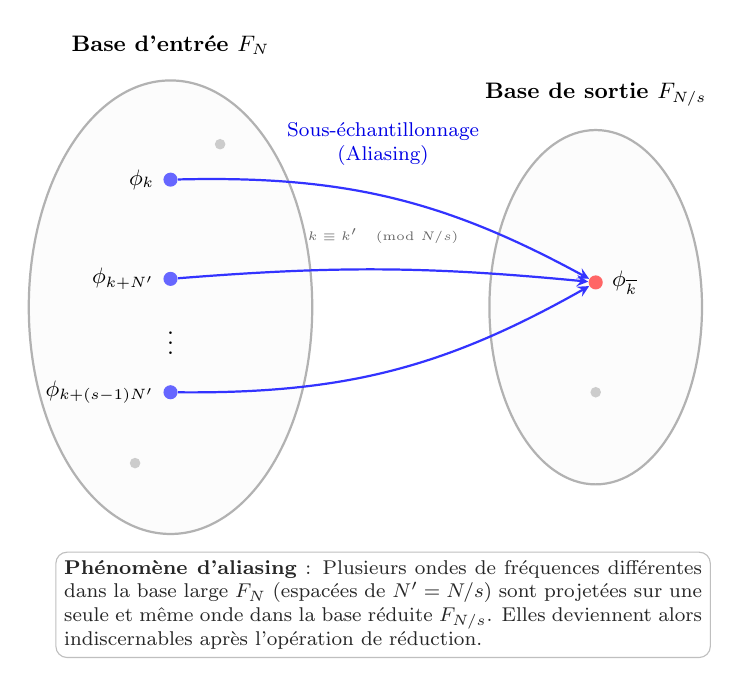
\begin{tikzpicture}[scale=0.9, transform shape]
        % --- ENSEMBLES (Patates) ---
        \draw[thick, gray!60, fill=gray!2] (0,0) ellipse (2cm and 3.2cm);
        \draw[thick, gray!60, fill=gray!2] (6,0) ellipse (1.5cm and 2.5cm);

        % Titres des ensembles
        \node[font=\small\bfseries] at (0, 3.7) {Base d'entrée $F_N$};
        \node[font=\small\bfseries] at (6, 3) {Base de sortie $F_{N/s}$};

        % --- POINTS/ONDES D'ENTRÉE ---
        % Groupe d'aliasing vers k_bar
        \node[circle, fill=blue!60, inner sep=2pt, label=left:{\small $\phi_k$}] (k1) at (0, 1.8) {};
        \node[circle, fill=blue!60, inner sep=2pt, label=left:{\small $\phi_{k+N'}$}] (k2) at (0, 0.4) {};
        
        % Points de suspension
        \node at (0, -0.4) {$\vdots$};
        
        \node[circle, fill=blue!60, inner sep=2pt, label=left:{\small $\phi_{k+(s-1)N'}$}] (k3) at (0, -1.2) {};
        
        % Autres points pour le style
        \node[circle, fill=gray!40, inner sep=1.5pt] (o1) at (0.7, 2.3) {};
        \node[circle, fill=gray!40, inner sep=1.5pt] (o2) at (-0.5, -2.2) {};

        % --- POINT DE SORTIE ---
        \node[circle, fill=red!60, inner sep=2pt, label=right:{\small $\phi_{\overline{k}}$}] (kout) at (6, 0.35) {};
        
        % Autre point de sortie
        \node[circle, fill=gray!40, inner sep=1.5pt] (oout) at (6, -1.2) {};

        % --- FLÈCHES (PROJECTION) ---
        \draw[->, >=stealth, thick, blue!80, bend left=15] (k1) to (kout);
        \draw[->, >=stealth, thick, blue!80, bend left=5] (k2) to (kout);
        \draw[->, >=stealth, thick, blue!80, bend right=15] (k3) to (kout);

        % Annotations (Positionnement corrigé pour éviter les collisions)
        \node[text=blue!90!black, font=\footnotesize, align=center] at (3, 2.3) {Sous-échantillonnage \\ (Aliasing)};
        \node[text=black!60, font=\tiny] at (3, 1.0) {$k \equiv k' \pmod{N/s}$};

        % Légende explicative en bas
        \node[draw=gray!50, rounded corners, fill=white, text=black!85, font=\footnotesize, text width=9cm, align=justify] at (3, -4.2) {
            \textbf{Phénomène d'aliasing} : Plusieurs ondes de fréquences différentes dans la base large $F_N$ 
            (espacées de $N'=N/s$) sont projetées sur une seule et même onde dans la base réduite $F_{N/s}$. 
            Elles deviennent alors indiscernables après l'opération de réduction.
        };

    \end{tikzpicture}
    \caption{Représentation ensembliste du repliement de spectre généralisé. Les flèches illustrent la perte d'injectivité : un ensemble de $s$ fréquences sources contribue à une unique fréquence de sortie.}
    \label{fig:aliasing_mapping}
\end{figure}

\paragraph{Pourquoi les résultats précédents ne s'appliquent plus directement}

Les résultats précédents reposaient sur le fait qu'une convolution circulaire de stride $1$
préserve la taille spatiale et agit séparément sur chaque fréquence de Fourier. Cette séparation
permet d'obtenir des vecteurs singuliers associés à une seule fréquence. Dès qu'une couche réduit
la résolution spatiale, cette propriété disparaît : le sous-échantillonnage regroupe plusieurs
fréquences d'entrée dans une même fréquence de sortie. C'est ce regroupement, ou aliasing,
que nous allons maintenant formaliser.

\subsection{Sous-échantillonnage spatial et aliasing fréquentiel}

Pour simplifier l'analyse nous allons commencer par isoler l'effet du sous-échantillonnage, indépendamment de toute convolution.
On suppose que $s$ divise $N$, et on note
\[
    N' = \frac{N}{s}.
\]
On définit l'opérateur de sous-échantillonnage
\[
    P_s : \mathbb{C}^N \longrightarrow \mathbb{C}^{N'}
\]
par
\begin{equation*}
    (P_s x)_r = x_{sr},
    \qquad r = 0,\dots,N'-1.
\end{equation*}
Autrement dit, $P_s$ conserve une valeur toutes les $s$ positions.

Soit maintenant $(F_N)_k$ une direction de Fourier 1D de taille $N$. En appliquant $P_s$ à cette
direction, on obtient, pour tout $r=0,\dots,N'-1$,
\begin{align*}
    \big(P_s (F_N)_k\big)_r
    &= ((F_N)_k)_{sr} \notag \\
    &= \frac{1}{\sqrt{N}}
       \exp\left(2\pi i \frac{k sr}{N}\right) \notag \\
    &= \frac{1}{\sqrt{N}}
       \exp\left(2\pi i \frac{k r}{N'}\right).
\end{align*}
Or l'exponentielle précédente dépend de $k$ modulo $N'$. En notant
\[
    \overline{k} = k \bmod N',
\]
et comme $N=sN'$, donc
\[
    \frac{1}{\sqrt{N}} = \frac{1}{\sqrt{s}}\frac{1}{\sqrt{N'}},
\]
on obtient
\begin{equation}
    P_s (F_N)_k
    =
    \frac{1}{\sqrt{s}}(F_{N'})_{\overline{k}}.
    \label{eq:sous_echantillonnage_fourier_1d}
\end{equation}

Ce qui signifie qu'après sous-échantillonnage, la fréquence $k$ de taille $N$ devient la fréquence $\overline{k}$ de taille $N'$.
En effet, cette équation exprime précisément le phénomène d'\textit{aliasing}. Deux fréquences $k$ et $k'$
telles que
\[
    k \equiv k' \pmod{N'}
\]
deviennent identiques après sous-échantillonnage.
Ainsi, pour chaque fréquence $\overline{k} \in \{0,\dots,N'-1\}$, il existe un ensemble de $s$ fréquences sources
dans le signal original,
\[
    \mathcal{A}_k
    =
    \left\{ \overline{k} + qN' \mid q \in \{0,\dots,s-1\} \right\},
\]
qui deviennent indistinguables après sous-échantillonnage !

Autrement dit, l'opérateur de sous-échantillonnage n'est pas \textbf{injectif} dans le domaine fréquentiel : 
$s$ fréquences distinctes de l'espace de départ, espacées de $N'$, se projettent sur une unique fréquence dans 
l'espace d'arrivée.

\paragraph{Extension au cas bidimensionnel.}

On étend maintenant ce raisonnement aux images de taille $N \times N$. On définit l'opérateur de
sous-échantillonnage spatial 2D
\[
    P_s^{(2D)} : \mathbb{C}^{N \times N} \longrightarrow \mathbb{C}^{N' \times N'}
\]
par
\begin{equation}
    \big(P_s^{(2D)}X\big)_{r,t}
    =
    X_{sr,st},
    \qquad r,t = 0,\dots,N'-1.
    \label{eq:def_sous_echantillonnage_2d}
\end{equation}
Il conserve donc une ligne sur $s$ et une colonne sur $s$.

Après vectorisation, on note $\Pi_s$ la matrice associée à l'opérateur
$P_s^{(2D)}$. Pour la direction de Fourier vectorisée
\[
    q_{u,v}
    =
    (F_N)_v \otimes (F_N)_u,
\]
on peut appliquer le résultat 1D sur chacune des deux dimensions. En utilisant le résultat
1D obtenu en \eqref{eq:sous_echantillonnage_fourier_1d} sur chacune des deux dimensions, on a
\begin{align}
    \Pi_s q_{u,v}
    &=
    \Pi_s\big((F_N)_v \otimes (F_N)_u\big) \notag \\
    &=
    \big(P_s(F_N)_v\big) \otimes \big(P_s(F_N)_u\big) \notag \\
    &=
    \left(\frac{1}{\sqrt{s}}(F_{N'})_{\overline{v}}\right)
    \otimes
    \left(\frac{1}{\sqrt{s}}(F_{N'})_{\overline{u}}\right) \notag \\
    &=
    \frac{1}{s}
    (F_{N'})_{\overline{v}} \otimes (F_{N'})_{\overline{u}}.
    \label{eq:sous_echantillonnage_fourier_2d}
\end{align}
où
\[
    \overline{u} = u \bmod N',
    \qquad
    \overline{v} = v \bmod N'.
\]

Ainsi, deux fréquences 2D $(u,v)$ et $(u',v')$ deviennent indistinguables après sous-échantillonnage
dès lors que
\[
    u \equiv u' \pmod{N'},
    \qquad
    v \equiv v' \pmod{N'}.
\]
Pour chaque fréquence de sortie $(\overline{u},\overline{v})$, l'ensemble des fréquences d'entrée qui
se projettent sur elle est donc
\begin{equation}
    \mathcal{A}_{\overline{u},\overline{v}}
    =
    \left\{
        (\overline{u}+q_1N',\,\overline{v}+q_2N')
        \;\middle|\;
        q_1,q_2 \in \{0,\dots,s-1\}
    \right\}.
    \label{eq:classe_aliasing_2d}
\end{equation}

\subsection{Convolution avec stride et repliement spectral}

Revenons maintenant au cas d'une couche convolutionnelle. Une convolution avec stride $s$ peut être vue
comme une convolution classique de stride $1$, suivie d'un sous-échantillonnage spatial non commutatif. Après vectorisation,
si $M_h$ désigne l'opérateur associé à une convolution circulaire de stride $1$ par un noyau $h$, et si
$\Pi_s$ désigne la matrice de sous-échantillonnage associée à $P_s^{(2D)}$, alors l'opérateur de convolution
avec stride $s$ s'écrit
\begin{equation}
    M_h^{(s)}
    =
    \Pi_s M_h.
    \label{eq:conv_stride_sampling}
\end{equation}

Cette écriture signifie que l'on calcule d'abord toutes les valeurs de la convolution, puis que l'on ne conserve
que les positions dont les deux indices spatiaux sont des multiples de $s$.

Comme $M_h$ est une convolution circulaire de stride $1$, cette direction est une direction propre de
l'opérateur. En utilisant la diagonalisation rappelée en \eqref{eq:diagonalisation_conv_2d}, on a
\[
    M_h q_{u,v}
    =
    \lambda_{u,v} q_{u,v},
\]
où $\lambda_{u,v}$ est la valeur propre associée à la fréquence $(u,v)$.

En appliquant ensuite le sous-échantillonnage, et en utilisant
\eqref{eq:sous_echantillonnage_fourier_2d}, on obtient

\begin{align}
    M_h^{(s)} q_{u,v}
    &=
    \Pi_s M_h q_{u,v} \notag \\
    &=
    \lambda_{u,v}\Pi_s q_{u,v} \notag \\
    &=
    \frac{\lambda_{u,v}}{s}
    q_{\overline{u},\overline{v}}^{(N')},
    \label{eq:action_conv_stride_fourier}
\end{align}

où
\[
    q_{\overline{u},\overline{v}}^{(N')}
    =
    (F_{N'})_{\overline{v}} \otimes (F_{N'})_{\overline{u}}.
\]

avec
\[
    \overline{u}=u \bmod N',
    \qquad
    \overline{v}=v \bmod N'.
\]

L'équation \eqref{eq:action_conv_stride_fourier} montre que la convolution avec stride conserve une partie
de la structure de Fourier, mais avec une différence essentielle : plusieurs fréquences d'entrée peuvent être
envoyées vers la même fréquence de sortie. Plus précisément, toutes les fréquences appartenant à la même
classe d'aliasing
\[
    \mathcal{A}_{\overline{u},\overline{v}}
    =
    \left\{
        (\overline{u}+q_1N',\,\overline{v}+q_2N')
        \;\middle|\;
        q_1,q_2\in\{0,\dots,s-1\}
    \right\}
\]
se retrouvent associées à la même fréquence de sortie $(\overline{u},\overline{v})$.

Pour exprimer ce regroupement de manière matricielle, on introduit la matrice
\[
    \mathcal{S}_s \in \mathbb{C}^{N'^2 \times N^2},
\]
qui décrit le repliement spectral dans la base de Fourier. Ses colonnes correspondent aux fréquences
d'entrée $(u,v)$, et ses lignes aux fréquences de sortie $(\alpha,\beta)$. On définit
\begin{equation}
    (\mathcal{S}_s)_{(\alpha,\beta),(u,v)}
    =
    \begin{cases}
        \dfrac{1}{s},
        & \text{si } \alpha = u \bmod N'
        \text{ et } \beta = v \bmod N', \\[0.4em]
        0,
        & \text{sinon.}
    \end{cases}
    \label{eq:def_matrice_sampling_fourier}
\end{equation}

Ainsi, pour une fréquence d'entrée $(u,v)$ donnée, la matrice $\mathcal{S}_s$ place un unique coefficient
non nul sur la ligne correspondant à la fréquence de sortie
\[
    (u \bmod N',\, v \bmod N').
\]
Ce coefficient vaut $\frac{1}{s}$, comme dans \eqref{eq:sous_echantillonnage_fourier_2d}.

L'action du sous-échantillonnage sur toute la base de Fourier s'écrit alors
\begin{equation}
    \Pi_s Q_N
    =
    Q_{N'} \mathcal{S}_s.
    \label{eq:sampling_base_fourier}
\end{equation}
Comme $Q_N$ est unitaire, on obtient la factorisation
\begin{equation}
    \Pi_s
    =
    Q_{N'} \mathcal{S}_s Q_N^H.
    \label{eq:factorisation_sampling_fourier}
\end{equation}

Cette écriture confirme que $\mathcal{S}_s$ représente bien l'aliasing dans le domaine fréquentiel.
En effet, si
\[
    \widehat{x}=Q_N^H x
\]
désigne les coefficients de Fourier de l'entrée, alors les coefficients de Fourier de la sortie sous-échantillonnée
sont donnés par
\[
    \widehat{y}
    =
    Q_{N'}^H\Pi_s x
    =
    \mathcal{S}_s \widehat{x}.
\]
Par définition de $\mathcal{S}_s$, cela donne, pour chaque fréquence de sortie $(\alpha,\beta)$,
\begin{equation}
    \widehat{y}_{\alpha,\beta}
    =
    \frac{1}{s}
    \sum_{(u,v)\in\mathcal{A}_{\alpha,\beta}}
    \widehat{x}_{u,v}.
    \label{eq:somme_coefficients_aliasing}
\end{equation}

Autrement dit, le sous-échantillonnage ne conserve pas séparément les coefficients de Fourier :
il additionne les coefficients appartenant à une même classe d'aliasing. C'est ce mécanisme qui explique
pourquoi, dans une couche avec stride, les directions singulières ne sont plus nécessairement associées
à une seule fréquence de Fourier.

\subsection{Composition avec une convolution de stride $1$}

On peut maintenant combiner le sous-échantillonnage avec une convolution circulaire de stride $1$.
On considère une couche convolutionnelle multi-canaux de stride $1$, représentée par l'opérateur
matriciel $M$. D'après la factorisation établie en \eqref{eq:factorisation_M}, on a
\begin{equation*}
    M
    =
    (I_{m_{\mathrm{out}}} \otimes Q_N)
    L
    (I_{m_{\mathrm{in}}} \otimes Q_N)^H,
\end{equation*}

Une convolution avec stride $s$ s'obtient alors en appliquant d'abord la convolution de stride $1$,
puis en gardant seulement une position sur $s$ dans chaque direction spatiale. Comme cette réduction
est faite séparément sur chaque canal de sortie, on introduit
\[
    \Pi_s^{\mathrm{out}}
    =
    I_{m_{\mathrm{out}}} \otimes \Pi_s.
\]
L'opérateur correspondant à la convolution avec stride $s$ s'écrit alors
\begin{equation*}
    M^{(s)}
    =
    \Pi_s^{\mathrm{out}} M.
\end{equation*}

En remplaçant $M$ par sa factorisation de Fourier et $\Pi_s$ par la factorisation obtenue en
\eqref{eq:factorisation_sampling_fourier}, on obtient
\begin{align*}
    M^{(s)}
    &=
    (I_{m_{\mathrm{out}}} \otimes \Pi_s)
    (I_{m_{\mathrm{out}}} \otimes Q_N)
    L
    (I_{m_{\mathrm{in}}} \otimes Q_N)^H \notag \\
    &=
    (I_{m_{\mathrm{out}}} \otimes Q_{N'})
    (I_{m_{\mathrm{out}}} \otimes \mathcal{S}_s)
    L
    (I_{m_{\mathrm{in}}} \otimes Q_N)^H.
\end{align*}

Cette écriture montre clairement où apparaît la différence avec le cas stride $1$. Le facteur $L$
continue d'agir fréquence par fréquence. En revanche, le facteur $\mathcal{S}_s$ regroupe ensuite
plusieurs fréquences d'entrée dans une même fréquence de sortie.

Pour mieux voir ce regroupement, on reprend le même raisonnement que plus haut.
Soit

\begin{equation*}
    \widehat{x}_{u,v} \in \mathbb{C}^{m_{\mathrm{in}}}
    \qquad \text{et} \qquad
    \widehat{z}_{u,v} = G^{(u,v)} \widehat{x}_{u,v}.
\end{equation*}

On applique ensuite le sous-échantillonnage pour une fréquence réduite $(\alpha,\beta)$,
\begin{align}
    \widehat{y}_{\alpha,\beta}
    &=
    \frac{1}{s}
    \sum_{(u,v)\in\mathcal{A}_{\alpha,\beta}}
    \widehat{z}_{u,v} \notag \\
    &=
    \frac{1}{s}
    \sum_{(u,v)\in\mathcal{A}_{\alpha,\beta}}
    G^{(u,v)}\widehat{x}_{u,v}.
    \label{eq:sortie_stride_classe_aliasing}
\end{align}

Pour écrire cette relation sous forme matricielle, on fixe un ordre arbitraire sur les fréquences de
la classe d'aliasing :
\[
    \mathcal{A}_{\alpha,\beta}
    =
    \{(u_1,v_1),\dots,(u_{s^2},v_{s^2})\}.
\]
On regroupe ensuite les coefficients d'entrée correspondants dans un seul vecteur :
\[
    \widehat{x}_{\mathcal{A}_{\alpha,\beta}}
    =
    \begin{pmatrix}
        \widehat{x}_{u_1,v_1} \\
        \vdots \\
        \widehat{x}_{u_{s^2},v_{s^2}}
    \end{pmatrix}
    \in \mathbb{C}^{m_{\mathrm{in}}s^2}.
\]

On obtient alors la matrice
\begin{equation}
    G_s^{(\alpha,\beta)}
    =
    \frac{1}{s}
    \begin{pmatrix}
        G^{(u_1,v_1)}
        &
        G^{(u_2,v_2)}
        &
        \cdots
        &
        G^{(u_{s^2},v_{s^2})}
    \end{pmatrix}
    \in
    \mathbb{C}^{m_{\mathrm{out}}\times m_{\mathrm{in}}s^2}.
    \label{eq:def_matrice_aliasing_stride}
\end{equation}

Cette matrice est simplement une façon compacte d'écrire la somme de
\eqref{eq:sortie_stride_classe_aliasing}. En effet, multiplier
$G_s^{(\alpha,\beta)}$ par le vecteur empilé
$\widehat{x}_{\mathcal{A}_{\alpha,\beta}}$ donne exactement
\[
    \frac{1}{s}
    \sum_{(u,v)\in\mathcal{A}_{\alpha,\beta}}
    G^{(u,v)}\widehat{x}_{u,v}.
\]
On a donc par construction
\begin{equation*}
    \widehat{y}_{\alpha,\beta}
    =
    G_s^{(\alpha,\beta)}
    \widehat{x}_{\mathcal{A}_{\alpha,\beta}}.
\end{equation*}

Cette formulation permet de ramener l'étude de la sensibilité structurelle d'une convolution avec stride $s$ à 
une analyse locale, fréquence de sortie par fréquence de sortie. Pour chaque fréquence réduite $(\alpha,\beta)$, 
il convient alors d'étudier les valeurs et vecteurs singuliers de la matrice $G_s^{(\alpha,\beta)}$.

\subsection{Construction des vecteurs singuliers droits}

\begin{proof}

Pour alléger les notations, on pose
\[
    \varphi_{u,v}^{(N)}
    =
    (F_N)_v \otimes (F_N)_u,
    \qquad
    \varphi_{\alpha,\beta}^{(N')}
    =
    (F_{N'})_\beta \otimes (F_{N'})_\alpha.
\]

On fixe une fréquence de sortie $(\alpha,\beta)$ et sa classe d'aliasing
$\mathcal{A}_{\alpha,\beta}$. En choisissant un ordre arbitraire sur cette classe,
on écrit
\[
    \mathcal{A}_{\alpha,\beta}
    =
    \{(u_1,v_1),\dots,(u_{s^2},v_{s^2})\}.
\]
Soit
\[
    p
    =
    \begin{pmatrix}
        p_{u_1,v_1} \\
        \vdots \\
        p_{u_{s^2},v_{s^2}}
    \end{pmatrix}
    \in \mathbb{C}^{m_{\mathrm{in}}s^2},
    \qquad
    p_{u_i,v_i}\in\mathbb{C}^{m_{\mathrm{in}}},
\]
un vecteur singulier droit de $G_s^{(\alpha,\beta)}$, associé à une valeur singulière
$\sigma$ et à un vecteur singulier gauche $q\in\mathbb{C}^{m_{\mathrm{out}}}$. On a donc
\begin{equation}
    G_s^{(\alpha,\beta)}p
    =
    \sigma q,
    \qquad
    G_s^{(\alpha,\beta)H}q
    =
    \sigma p.
    \label{eq:svd_matrice_aliasing_stride}
\end{equation}

À partir des blocs $p_{u,v}$, on construit le vecteur d'entrée
\begin{equation}
    r
    =
    \sum_{(u,v)\in\mathcal{A}_{\alpha,\beta}}
    p_{u,v}\otimes \varphi_{u,v}^{(N)}.
    \label{eq:construction_vecteur_singulier_stride}
\end{equation}
Ce vecteur n'est donc plus associé à une seule fréquence de Fourier : c'est une combinaison
de toutes les fréquences appartenant à la même classe d'aliasing.

Montrons maintenant que $r$ est un vecteur singulier droit de $M^{(s)}$. D'après
\eqref{eq:sortie_stride_classe_aliasing}, l'action de $M^{(s)}$ sur les coefficients de Fourier
associés à la classe $\mathcal{A}_{\alpha,\beta}$ est donnée par
\[
    \widehat{y}_{\alpha,\beta}
    =
    \frac{1}{s}
    \sum_{(u,v)\in\mathcal{A}_{\alpha,\beta}}
    G^{(u,v)}p_{u,v}.
\]
Par définition de $G_s^{(\alpha,\beta)}$, cette somme s'écrit simplement
\[
    \widehat{y}_{\alpha,\beta}
    =
    G_s^{(\alpha,\beta)}p.
\]
En utilisant la relation de singularité \eqref{eq:svd_matrice_aliasing_stride}, on obtient donc
\[
    \widehat{y}_{\alpha,\beta}
    =
    \sigma q.
\]
Dans le domaine spatial, cela donne
\[
    M^{(s)}r
    =
    \sigma q\otimes \varphi_{\alpha,\beta}^{(N')}.
\]
En posant
\[
    w
    =
    q\otimes \varphi_{\alpha,\beta}^{(N')},
\]
on obtient
\begin{equation}
    M^{(s)}r = \sigma w.
    \label{eq:relation_singuliere_stride_droite}
\end{equation}

Il reste à vérifier l'équation adjointe. L'adjoint de $M^{(s)}$ renvoie une fréquence de sortie
$(\alpha,\beta)$ vers toutes les fréquences d'entrée de la classe
$\mathcal{A}_{\alpha,\beta}$. On obtient alors
\[
    M^{(s)H}w
    =
    \sum_{(u,v)\in\mathcal{A}_{\alpha,\beta}}
    \frac{1}{s}
    \left(
        G^{(u,v)H}q
    \right)
    \otimes
    \varphi_{u,v}^{(N)}.
\]
Or la relation
\[
    G_s^{(\alpha,\beta)H}q=\sigma p
\]
implique, bloc par bloc, que
\[
    \frac{1}{s}G^{(u,v)H}q
    =
    \sigma p_{u,v},
    \qquad
    (u,v)\in\mathcal{A}_{\alpha,\beta}.
\]
En remplaçant dans l'expression précédente, on obtient directement
\begin{equation}
    M^{(s)H}w
    =
    \sigma r.
    \label{eq:relation_singuliere_stride_gauche}
\end{equation}

Les deux relations
\[
    M^{(s)}r=\sigma w,
    \qquad
    M^{(s)H}w=\sigma r
\]
montrent donc que $r$ et $w$ forment bien une paire de vecteurs singuliers droit et gauche
de $M^{(s)}$.

Enfin, la normalisation est conservée. En effet, les fréquences de
$\mathcal{A}_{\alpha,\beta}$ sont distinctes, donc les directions
$\varphi_{u,v}^{(N)}$ correspondantes sont orthonormées. Ainsi,
\[
    \|r\|_2^2
    =
    \sum_{(u,v)\in\mathcal{A}_{\alpha,\beta}}
    \|p_{u,v}\|_2^2
    =
    \|p\|_2^2.
\]
Donc si $p$ est normalisé, alors $r$ l'est aussi. De même, si $q$ est normalisé,
alors $w=q\otimes \varphi_{\alpha,\beta}^{(N')}$ est normalisé.

On retrouve ainsi le résultat annoncé par la Proposition~5 de Tsuzuku et Sato
\cite{tsuzuku2019structural} : dans une couche de réduction, les directions singulières
ne sont plus forcément des directions de Fourier pures. Elles peuvent être des combinaisons
de fréquences appartenant à une même classe d'aliasing.

\end{proof}

\subsection{Average pooling comme cas particulier}

L'\textit{average pooling} consiste à remplacer chaque fenêtre locale de taille $s\times s$
par la moyenne de ses pixels comme illustré dans la Figure~\ref{fig:avg_pooling_spatial}. Cette opération réduit donc la résolution spatiale, comme une
convolution avec stride. La différence est qu'avant le sous-échantillonnage, on applique d'abord
un filtre moyenneur fixe.

Dans le cadre circulaire utilisé ici, ce filtre peut être représenté par le noyau
\[
    h_{\mathrm{avg}}[a,b]
    =
    \begin{cases}
        \dfrac{1}{s^2},
        & \text{si } a,b \in \{0,\dots,s-1\},\\[0.4em]
        0,
        & \text{sinon,}
    \end{cases}
\]
où les indices spatiaux sont interprétés modulo $N$. La convolution par
$h_{\mathrm{avg}}$ calcule donc une moyenne locale, puis le sous-échantillonnage conserve
une position sur $s$ dans chaque direction spatiale.

Dans le cas multi-canaux, cette opération est appliquée séparément sur chaque canal. Si $m$
désigne le nombre de canaux et si
$C_{h_{\mathrm{avg}}}\in\mathbb{C}^{N^2\times N^2}$ désigne la matrice de convolution circulaire
associée au noyau moyenneur, alors l'opérateur d'\textit{average pooling} s'écrit
\begin{equation}
    M_{\mathrm{avg}}^{(s)}
    =
    (I_m \otimes \Pi_s)
    (I_m \otimes C_{h_{\mathrm{avg}}}).
    \label{eq:average_pooling_convolution_sampling}
\end{equation}

On est donc exactement dans le cas étudié précédemment : une convolution circulaire de stride $1$,
suivie d'un sous-échantillonnage. Le noyau moyenneur agit comme un filtre passe-bas, ce qui atténue
certaines fréquences avant le repliement spectral. Mais le mécanisme d'aliasing reste le même :
plusieurs fréquences d'entrée peuvent être regroupées dans une même fréquence de sortie.

Par conséquent, les vecteurs singuliers droits d'une couche d'\textit{average pooling} peuvent eux aussi
être choisis comme des combinaisons de fréquences appartenant à une même classe d'aliasing.

\section{Contrainte image réelle}
\label{sec:contrainte-image-reelle}

La Proposition~6 de Tsuzuku et Sato~\cite{tsuzuku2019structural} vise à résoudre le problème lié à l'utilisation des 
méthodes que nous venons de développer dans des cas concrets. En effet, les images manipulées par un réseau sont réelles, 
tandis qu'une fonction de Fourier prise isolément est en général complexe. L'idée est de montrer que la contrainte de 
valeur réelle d'une image peut être résolue en utilisant la symétrie hermitienne de ses coefficients de Fourier. Et pour cela nous allons 
introduire les outils nécessaires pour comprendre cette symétrie.

Commencons par la transformée de Fourier discrète 2D~\cite{ImagerieNumeriqueTheme7Block2}. Pour une image
$X\in\mathbb{C}^{N\times N}$, on définit
\begin{equation*}
    \widehat{X}_{u,v}
    =
    S(X)_{u,v}
    =
    \sum_{m=0}^{N-1}\sum_{n=0}^{N-1}
    X[m,n]\,
    \exp\left(
        -2\pi i\frac{um+vn}{N}
    \right),
    \qquad
    u,v\in\{0,\dots,N-1\}.
\end{equation*}

L'image peut être reconstruite à partir de ses coefficients de Fourier par la transformée inverse :
\begin{equation}
    X[m,n]
    =
    \frac{1}{N^2}
    \sum_{u=0}^{N-1}\sum_{v=0}^{N-1}
    \widehat{X}_{u,v}\,
    \exp\left(
        2\pi i\frac{um+vn}{N}
    \right).
    \label{eq:idft2d_definition}
\end{equation}

Ces formules sont compatibles avec les bases de Fourier introduites précédemment, à un facteur de
normalisation près. Ici, nous suivons la notation $S(X)$ utilisée dans l'article \cite{tsuzuku2019structural} afin de reproduire
directement la Proposition~6.

\subsection{Symétrie hermitienne des coefficients de Fourier}

La contrainte de valeur réelle d'une image se traduit par une symétrie particulière de ses coefficients de
Fourier. Plus précisément, pour une image $X\in\mathbb{C}^{N\times N}$, on a
\begin{equation}
    X\in\mathbb{R}^{N\times N}
    \quad\Longleftrightarrow\quad
    \widehat{X}_{u,v}
    =
    \widehat{X}^{*}_{(-u)\bmod N,\,(-v)\bmod N},
    \qquad
    u,v\in\{0,\dots,N-1\}.
    \label{eq:symetrie_hermitienne_fourier}
\end{equation}
Cette propriété est la symétrie hermitienne de la transformée de Fourier d'un signal réel. Elle est
classique en traitement du signal discret~\cite{oppenheim2009discrete}, et correspond ici à la
Proposition~6 de Tsuzuku et Sato~\cite{tsuzuku2019structural}.

Montrons d'abord le sens direct. Supposons que $X$ soit réelle, c'est-à-dire que
\[
    X[m,n]^* = X[m,n]
    \qquad
    \text{pour tout } m,n.
\]
Par définition de la DFT 2D, on a
\begin{align*}
    \widehat{X}^{*}_{u,v}
    &=
    \left(
        \sum_{m=0}^{N-1}\sum_{n=0}^{N-1}
        X[m,n]\,
        \exp\left(-2\pi i\frac{um+vn}{N}\right)
    \right)^* \notag \\
    &=
    \sum_{m=0}^{N-1}\sum_{n=0}^{N-1}
    X[m,n]^*\,
    \exp\left(2\pi i\frac{um+vn}{N}\right) \notag \\
    &=
    \sum_{m=0}^{N-1}\sum_{n=0}^{N-1}
    X[m,n]\,
    \exp\left(-2\pi i\frac{((-u)m+(-v)n)}{N}\right) \notag \\
    &=
    \widehat{X}_{(-u)\bmod N,\,(-v)\bmod N}.
\end{align*}
On obtient donc bien
\[
    \widehat{X}_{u,v}
    =
    \widehat{X}^{*}_{(-u)\bmod N,\,(-v)\bmod N}.
\]

Prouvons maintenant le sens inverse. Supposons que les coefficients de Fourier vérifient la symétrie
\eqref{eq:symetrie_hermitienne_fourier}. On veut montrer que l'image reconstruite est réelle.
À partir de la transformée de Fourier inverse \eqref{eq:idft2d_definition}, on calcule le conjugué
de $X[m,n]$ :
\begin{align*}
    X[m,n]^*
    &=
    \left(
        \frac{1}{N^2}
        \sum_{u=0}^{N-1}\sum_{v=0}^{N-1}
        \widehat{X}_{u,v}
        \exp\left(2\pi i\frac{um+vn}{N}\right)
    \right)^* \notag \\
    &=
    \frac{1}{N^2}
    \sum_{u=0}^{N-1}\sum_{v=0}^{N-1}
    \widehat{X}^{*}_{u,v}
    \exp\left(-2\pi i\frac{um+vn}{N}\right).
\end{align*}
Pour rappel d'après l'hypothèse de symétrie hermitienne, on a
\[
    \widehat{X}^{*}_{u,v}
    =
    \widehat{X}_{(-u)\bmod N,\,(-v)\bmod N}.
\]
Donc
\begin{align*}
    X[m,n]^*
    &=
    \frac{1}{N^2}
    \sum_{u=0}^{N-1}\sum_{v=0}^{N-1}
    \widehat{X}_{(-u)\bmod N,\,(-v)\bmod N}
    \exp\left(-2\pi i\frac{um+vn}{N}\right).
\end{align*}
En effectuant le changement d'indices
\[
    u' = (-u)\bmod N,
    \qquad
    v' = (-v)\bmod N,
\]
on obtient
\begin{align*}
    X[m,n]^*
    &=
    \frac{1}{N^2}
    \sum_{u'=0}^{N-1}\sum_{v'=0}^{N-1}
    \widehat{X}_{u',v'}
    \exp\left(2\pi i\frac{u'm+v'n}{N}\right) \notag \\
    &=
    X[m,n].
\end{align*}
Ainsi $X[m,n]^*=X[m,n]$ pour tout $m,n$, donc $X$ est réelle.

On a donc bien montré l'équivalence :
\[
    X\in\mathbb{R}^{N\times N}
    \quad\Longleftrightarrow\quad
    \widehat{X}_{u,v}
    =
    \widehat{X}^{*}_{(-u)\bmod N,\,(-v)\bmod N}.
\]

\subsection{Conséquence pour les perturbations de Fourier}

L'équivalence précédente s'applique directement aux perturbations que l'on souhaite ajouter aux images.
Comme les images manipulées par le réseau sont réelles,
\[
    x \in \mathbb{R}^{N\times N\times c},
\]
une perturbation admissible doit elle aussi être réelle dans le domaine spatial. Ainsi, pour chaque canal,
ses coefficients de Fourier doivent vérifier la symétrie hermitienne :
\begin{equation}
    \widehat{\delta}_{(-u)\bmod N,\,(-v)\bmod N}
    =
    \widehat{\delta}_{u,v}^{*}.
    \label{eq:contrainte_reelle_perturbation_fourier}
\end{equation}

Autrement dit, si l'on utilise une fréquence \((u,v)\), il faut aussi utiliser sa fréquence opposée
\[
    ((-u)\bmod N,\,(-v)\bmod N)
\]
avec le coefficient conjugué. Cette condition garantit que la transformée inverse de Fourier donne une perturbation réelle.

Il existe quelques cas particuliers où une fréquence est égale à sa propre fréquence opposée modulo $N$.
Ces fréquences vérifient
\[
    (u,v)
    =
    ((-u)\bmod N,\,(-v)\bmod N).
\]
Dans ce cas, la condition précédente impose simplement que le coefficient de Fourier soit réel. Pour
$N$ pair, cela concerne notamment les fréquences
\[
    (0,0),
    \qquad
    (N/2,0),
    \qquad
    (0,N/2),
    \qquad
    (N/2,N/2).
\]
En dehors de ces cas particuliers, les fréquences doivent être prises par paires conjuguées.

C'est cette idée qui est utilisée par Tsuzuku et Sato dans leur \textit{Single Fourier Attack}
\cite{tsuzuku2019structural}. 
Pour une fréquence non auto-conjuguée, une perturbation de type \textit{Single Fourier Attack}
peut alors s'écrire sous la forme
\begin{equation}
    \delta_{u,v}
    =
    \eta
    \left[
        (1+i)\,q_{u,v}
        +
        (1-i)\,q_{(-u)\bmod N,\,(-v)\bmod N}
    \right].
    \label{eq:sfa_perturbation_fourier}
\end{equation}

Les coefficients $(1+i)$ et $(1-i)$ sont conjugués l'un de l'autre, et les deux directions de Fourier
correspondent à des fréquences opposées. La perturbation respecte donc la condition
\eqref{eq:contrainte_reelle_perturbation_fourier}, ce qui garantit qu'elle est réelle dans le domaine spatial.

Le paramètre $\eta$ règle l'amplitude de la perturbation dans cette écriture théorique. En pratique,
dans les expériences adversariales, on impose plutôt une borne sur les pixels, par exemple
\[
    \|\delta\|_\infty \leq \varepsilon.
\]

\section{Limites et portée du cadre théorique}

Les résultats précédents donnent une explication mathématique claire de la place particulière
des directions de Fourier dans les réseaux convolutionnels. Il faut toutefois préciser la portée
exacte de ce résultat.

\subsection{Un résultat exact dans un cadre contrôlé}

Le raisonnement précédent est exact dans un cadre précis : convolutions circulaires, couches
linéaires, et analyse de la sensibilité par valeurs singulières. Sous ces hypothèses, la
factorisation donnée en \eqref{eq:factorisation_M} permet d'étudier le réseau fréquence par
fréquence. Les directions singulières obtenues sont alors de la forme
\[
    a \otimes q_{u,v},
\]
où $q_{u,v}$ décrit le motif spatial de Fourier et $a$ le mélange entre les canaux.

Ce résultat doit donc être compris comme une propriété structurelle des convolutions, et non
comme une description complète d'un CNN réel.

\subsection{Écart avec les architectures réelles}

Les architectures utilisées en pratique s'écartent de ce cadre exact. Le \textit{zero-padding}
remplace souvent le padding circulaire, ce qui empêche une diagonalisation exacte par la base
de Fourier. Les couches de réduction, comme les convolutions avec stride et l'\textit{average
pooling}, introduisent un phénomène d'aliasing, déjà discuté dans la
section~\ref{sec:couches-reduction-stride-pooling}.

Enfin, les activations ReLU et le \textit{max-pooling} rendent le réseau non linéaire. Le réseau
complet ne peut donc plus être vu comme un unique opérateur linéaire diagonalisable par Fourier.
Cependant, ces opérations possèdent une structure linéaire par morceaux, ce qui permet de
conserver une interprétation locale de l'analyse fréquentielle.

\subsection{Portée locale de l'analyse fréquentielle dans les CNN non linéaires}

Dans cette sous-section, on considère que $f$ désigne l'application réalisée par le réseau
jusqu'aux logits, avant l'opération finale d'\textit{argmax} qui n'est pas une application affine.

Les réseaux utilisant des activations linéaires par morceaux, comme ReLU, peuvent être vus
comme des fonctions affines par morceaux : l'espace d'entrée est découpé en régions, et sur
chacune de ces régions, le réseau réalise une application affine~\cite{montufar2014number,balestriero2018spline}.
Cette observation permet de préciser la portée de l'analyse fréquentielle dans les CNN réels :
le réseau complet n'est pas globalement linéaire, mais son comportement peut être décrit
localement par une application affine tant que les choix d'activation et de pooling restent fixés.

Ce qui m'amène à la proposition suivante :

\begin{proposition}[Linéarisation locale d'un CNN avec ReLU et max-pooling]
Soit $f$ un réseau convolutionnel composé de couches convolutives, d'activations ReLU et de
couches de max-pooling. Pour toute entrée $x$ ne se trouvant pas
sur une frontière de changement de région linéaire, c'est-à-dire lorsque les signes des
pré-activations ReLU sont non nuls et que les maxima sélectionnés dans les fenêtres de pooling
sont uniques, il existe un voisinage $\mathcal{V}_x$ de $x$ tel que, pour tout
$z \in \mathcal{V}_x$,
\[
    f(z) = A_x z + b_x,
\]
où $A_x$ est une matrice dépendant de la région linéaire contenant $x$.
\end{proposition}

\begin{proof}
Une activation ReLU agit coordonnée par coordonnée selon
\[
    \mathrm{ReLU}(t)=\max(t,0).
\]
Considérons une couche donnée du réseau, et notons $a_\ell$ son vecteur de pré-activations.
Si le signe de chaque coordonnée de $a_\ell$ est fixé dans un voisinage de $x$, alors la ReLU
agit comme une application linéaire sur cette région :
\[
    \mathrm{ReLU}(a_\ell)=D_\ell(x)a_\ell,
\]
où $D_\ell(x)$ est une matrice diagonale dont les coefficients valent $0$ ou $1$ selon que les
coordonnées correspondantes sont désactivées ou activées.

De même, une couche de max-pooling sélectionne, dans chaque fenêtre locale, la coordonnée
de valeur maximale. Lorsque ce maximum est unique dans chaque fenêtre, les indices sélectionnés
restent inchangés dans un voisinage suffisamment petit de $x$. Dans cette région, le max-pooling
devient donc une application linéaire de sélection :
\[
    \mathrm{MaxPool}(z)=P_\ell(x)z,
\]
où $P_\ell(x)$ est une matrice de sélection dépendant de la région considérée. Cette matrice
encode à la fois le choix des maxima locaux et la réduction spatiale induite par le pooling.

Ainsi, tant que l'on reste dans une région où les signes des ReLU et les indices sélectionnés
par le max-pooling ne changent pas, chaque opération du réseau est affine ou linéaire. La
composition de ces opérations est donc elle-même affine. Il existe donc une matrice $A_x$ et un
vecteur $b_x$ tels que
\[
    f(z)=A_xz+b_x.
\]

Cette région locale peut être comprise comme l'ensemble des entrées pour lesquelles les masques 
d'activation ReLU et les indices sélectionnés par les couches de max-pooling restent inchangés.
\footnote{Une étude plus détaillée pourrait consister à définir explicitement cette région, 
par exemple comme l'ensemble des points (z) vérifiant les mêmes signes de pré-activation 
ReLU et les mêmes indices de maximum dans les fenêtres de pooling que l'entrée (x). 
L'analyse de la taille de cette région donnerait une mesure plus précise de la validité 
locale de la linéarisation, mais dépasse le cadre de ce travail.}

\end{proof}

Cette proposition montre qu'un CNN composé de convolutions, de ReLU et de max-pooling est
affine par morceaux. Autour d'une entrée $x$, tant que la perturbation ne change pas les masques d'activation ni les positions sélectionnées
par le pooling, le comportement du réseau est exactement linéaire à un biais près. Ainsi, pour
tout $x+\delta\in\mathcal{V}_x$, on a
\[
    f(x+\delta)-f(x)=J_f(x)\delta.
\]

Dans une telle région, le jacobien peut être vu comme un produit de matrices associées aux
différentes opérations du réseau. Par exemple, dans le cas schématique d'un empilement de blocs
convolution--ReLU--pooling, on peut écrire
\[
    J_f(x)
    =
    W_L P_{L-1}(x)D_{L-1}(x)M_{L-1}
    \cdots
    P_1(x)D_1(x)M_1,
\]
où les matrices $M_\ell$ représentent les convolutions, les matrices $D_\ell(x)$ les masques
ReLU, les matrices $P_\ell(x)$ les sélections induites par le max-pooling, et $W_L$ la partie
linéaire finale.

Les matrices $D_\ell(x)$ et $P_\ell(x)$ dépendent de l'entrée. Elles empêchent donc, en général,
une diagonalisation globale du réseau dans la base de Fourier. Une direction de Fourier n'est
plus un vecteur propre exact de l'application complète.

Cependant, les opérateurs convolutionnels $M_\ell$ restent présents dans le produit du
jacobien. L'analyse fréquentielle conserve donc une portée locale : elle ne décrit plus exactement
le réseau global, mais elle peut encore expliquer pourquoi certaines fréquences sont davantage
amplifiées que d'autres autour de certaines entrées.

On peut alors interpréter la \textit{Single Fourier Attack} comme une exploitation empirique de
cette sensibilité locale. Cette lecture prolonge l'hypothèse de linéarité de Goodfellow et
al.~\cite{goodfellow2015explaining}.

\subsection{Portée réelle du résultat}

Le cadre théorique ne permet pas de prédire exactement quelles fréquences seront les plus
sensibles pour une architecture donnée. Cette sensibilité dépend aussi des poids appris, du jeu
de données, du padding, des normalisations, des non-linéarités et des couches de réduction.

En revanche, l'analyse explique pourquoi les directions de Fourier constituent des candidates
naturelles : elles apparaissent directement dans l'étude linéaire des convolutions. Même dans un
CNN non linéaire, cette structure peut rester partiellement visible à travers le jacobien local du
modèle. La partie expérimentale servira donc à vérifier dans quelle mesure cette intuition reste
observable en pratique.

% \section{Lien avec les perturbations adversariales universelles}

% Le chapitre de contexte a introduit les perturbations adversariales universelles comme des
% perturbations capables d'affecter plusieurs images différentes. Le cadre théorique développé ici
% donne une explication possible à ce phénomène dans le cas des réseaux convolutionnels.

% Dans le modèle linéaire idéalisé, certaines directions de Fourier peuvent être fortement
% amplifiées par les couches convolutionnelles. Une perturbation construite sur une telle fréquence
% peut donc exploiter une sensibilité liée à la structure du réseau plutôt qu'à une image particulière.

% C'est cette idée qui motive la \textit{Single Fourier Attack} de Tsuzuku et
% Sato~\cite{tsuzuku2019structural}. Au lieu de chercher une perturbation libre dans tout l'espace
% des pixels, l'attaque restreint la recherche à une fréquence de Fourier. Dans un CNN réel, cette
% sensibilité n'est plus une propriété exacte globale, mais elle peut rester visible localement et en
% moyenne sur les images.

% La suite du travail consiste donc à construire des cartes de sensibilité fréquentielle afin
% d'observer quelles fréquences affectent réellement le modèle étudié.